\documentclass[12pt]{article}
\makeatletter\if@twocolumn\PassOptionsToPackage{switch}{lineno}\else\fi\makeatother

  
\usepackage{mathtools,amsmath,amsfonts,amsbsy,tabulary,longtable,rotating, makecell,graphicx,times,caption,subcaption,fancyhdr,chngcntr}
\usepackage[utf8]{inputenc}
\usepackage[paperheight=11in,paperwidth=8.5in,margin=1in]{geometry}
\usepackage[title]{appendix}
\renewenvironment{abstract} {\vspace*{-1pc}\trivlist\item[]\leftskip\oupIndent\par\vskip4pt\noindent\textbf{\abstractname}\mbox{\null}\\\relax}{\par\noindent\endtrivlist}
\renewcommand\cellalign{cc}
\linespread{1.5} \date{}
\captionsetup[figure]{labelfont=sc,skip=1.4pt,aboveskip=1pc}
\captionsetup[table]{labelfont=sc,skip=1.4pt,labelsep=newline}



\makeatletter\def\oupIndent{1pt}
\def\author#1{\gdef\@author{\hskip-\dimexpr(\tabcolsep)\hskip\oupIndent\parbox{\dimexpr\textwidth-\oupIndent}{\centering\raggedright\bfseries#1}}}
\def\title#1{\gdef\@title{\centering\raggedright\bfseries\ifx\@articleType\@empty\else\@articleType\\\fi#1}}
\let\@articleType\@empty \def\articletype#1{\gdef\@articleType{{\normalfont\itshape#1}}}
\fancypagestyle{headings}{\fancyhf{}\fancyhead[C]{\RunningHead}\fancyhead[R]{\thepage}}\pagestyle{headings}
%\setlength{\headheight}{52pt}
\makeatother
\raggedright 

\long\def\acknote#1{%
  \let\thempfn\relax% Remove footnote number printing mechanism
  \footnotetext[0]{{#1}}% Print footnote text
}
  


\tolerance=5000
%%%%%%%%%%%%%%%%%%%%%%%%%%%%%%%%%%%%%%%%%%%%%%%%%%%%%%%%%%%%%%%%%%%%%%%%%%
% Following additional macros are required to function some 
% functions which are not available in the class used.
%%%%%%%%%%%%%%%%%%%%%%%%%%%%%%%%%%%%%%%%%%%%%%%%%%%%%%%%%%%%%%%%%%%%%%%%%%
\usepackage{url,multirow,morefloats,floatflt,cancel,tfrupee}
\makeatletter


\AtBeginDocument{\@ifpackageloaded{textcomp}{}{\usepackage{textcomp}}}
\makeatother
\usepackage{colortbl}
\usepackage{xcolor}
\usepackage{pifont}
\usepackage[nointegrals]{wasysym}
\urlstyle{rm}
\makeatletter

%%%For Table column width calculation.
\def\mcWidth#1{\csname TY@F#1\endcsname+\tabcolsep}

%%Hacking center and right align for table
\def\cAlignHack{\rightskip\@flushglue\leftskip\@flushglue\parindent\z@\parfillskip\z@skip}
\def\rAlignHack{\rightskip\z@skip\leftskip\@flushglue \parindent\z@\parfillskip\z@skip}

%Etal definition in references
\@ifundefined{etal}{\def\etal{\textit{et~al}}}{}


%\if@twocolumn\usepackage{dblfloatfix}\fi
\usepackage{ifxetex}
\ifxetex\else\if@twocolumn\@ifpackageloaded{stfloats}{}{\usepackage{dblfloatfix}}\fi\fi

\AtBeginDocument{
\expandafter\ifx\csname eqalign\endcsname\relax
\def\eqalign#1{\null\vcenter{\def\\{\cr}\openup\jot\m@th
  \ialign{\strut$\displaystyle{##}$\hfil&$\displaystyle{{}##}$\hfil
      \crcr#1\crcr}}\,}
\fi
}

%For fixing hardfail when unicode letters appear inside table with endfloat
\AtBeginDocument{%
  \@ifpackageloaded{endfloat}%
   {\renewcommand\efloat@iwrite[1]{\immediate\expandafter\protected@write\csname efloat@post#1\endcsname{}}}{\newif\ifefloat@tables}%
}%

\def\BreakURLText#1{\@tfor\brk@tempa:=#1\do{\brk@tempa\hskip0pt}}
\let\lt=<
\let\gt=>
\def\processVert{\ifmmode|\else\textbar\fi}
\let\processvert\processVert

\@ifundefined{subparagraph}{
\def\subparagraph{\@startsection{paragraph}{5}{2\parindent}{0ex plus 0.1ex minus 0.1ex}%
{0ex}{\normalfont\small\itshape}}%
}{}

% These are now gobbled, so won't appear in the PDF.
\newcommand\role[1]{\unskip}
\newcommand\aucollab[1]{\unskip}
\newcommand{\GEZO}{Health Survey As Of 2014. [online] Available at: \textless https://www.cbs.nl/en-gb/our-services/methods/surveys/korte-onderzoeksbeschrijvingen/health-survey-as-of-2014\textgreater [Accessed 3 January 2021]}
  
\@ifundefined{tsGraphicsScaleX}{\gdef\tsGraphicsScaleX{1}}{}
\@ifundefined{tsGraphicsScaleY}{\gdef\tsGraphicsScaleY{.9}}{}
% To automatically resize figures to fit inside the text area
\def\checkGraphicsWidth{\ifdim\Gin@nat@width>\linewidth
	\tsGraphicsScaleX\linewidth\else\Gin@nat@width\fi}

\def\checkGraphicsHeight{\ifdim\Gin@nat@height>.9\textheight
	\tsGraphicsScaleY\textheight\else\Gin@nat@height\fi}

\def\fixFloatSize#1{}%\@ifundefined{processdelayedfloats}{\setbox0=\hbox{\includegraphics{#1}}\ifnum\wd0<\columnwidth\relax\renewenvironment{figure*}{\begin{figure}}{\end{figure}}\fi}{}}
\let\ts@includegraphics\includegraphics

\def\inlinegraphic[#1]#2{{\edef\@tempa{#1}\edef\baseline@shift{\ifx\@tempa\@empty0\else#1\fi}\edef\tempZ{\the\numexpr(\numexpr(\baseline@shift*\f@size/100))}\protect\raisebox{\tempZ pt}{\ts@includegraphics{#2}}}}

%\renewcommand{\includegraphics}[1]{\ts@includegraphics[width=\checkGraphicsWidth]{#1}}
\AtBeginDocument{\def\includegraphics{\@ifnextchar[{\ts@includegraphics}{\ts@includegraphics[width=\checkGraphicsWidth,height=\checkGraphicsHeight,keepaspectratio]}}}

\DeclareMathAlphabet{\mathpzc}{OT1}{pzc}{m}{it}

\def\URL#1#2{\@ifundefined{href}{#2}{\href{#1}{#2}}}

%%For url break
\def\UrlOrds{\do\*\do\-\do\~\do\'\do\"\do\-}%
\g@addto@macro{\UrlBreaks}{\UrlOrds}



\edef\fntEncoding{\f@encoding}
\def\EUoneEnc{EU1}
\makeatother
\def\floatpagefraction{0.8} 
\def\dblfloatpagefraction{0.8}
\def\style#1#2{#2}
\def\xxxguillemotleft{\fontencoding{T1}\selectfont\guillemotleft}
\def\xxxguillemotright{\fontencoding{T1}\selectfont\guillemotright}

\newif\ifmultipleabstract\multipleabstractfalse%
\newenvironment{typesetAbstractGroup}{}{}%

%%%%%%%%%%%%%%%%%%%%%%%%%%%%%%%%%%%%%%%%%%%%%%%%%%%%%%%%%%%%%%%%%%%%%%%%%%



%\usepackage[round,numbers,sort&compress]{natbib}
\usepackage[default]{jasa_harvard}    % 	for formatting citations in text
\renewcommand{\harvardand}{and}

\usepackage[T1]{fontenc}

\usepackage{float}

\begin{document}


\title{Optimal Stratification in Bayesian Adaptive Survey Designs}
\author{\textbf{\fontsize{14pt}{16.4pt}\selectfont{Yongchao Ma}}~\\\normalsize\normalfont {Department of Methodology and Statistics\unskip, Faculty of Social and Behavioral Sciences\unskip, Utrecht University\unskip, Heidelberglaan 8\unskip, Utrecht\unskip, 3584 CS\unskip, The Netherlands}~\\{\normalsize\normalfont  E-mail: y.ma1@uu.nl}}
\def\RunningHead{{Optimal Stratification in Bayesian Adaptive Survey Designs}}

\maketitle 
\acknote{}

\begin{abstract}
In an increasing number of survey designs, adaptive data collection strategies for different members of the population are adopted to balance the data quality and cost.
Stratifying the target population into subgroups in an effective manner plays a decisive role in identifying the optimal adaptive survey design.
This paper presents a stratification method on the basis of which the optimal adaptive survey designs can be constructed under the Bayesian analysis to minimize nonresponse bias.
The utility of this method compared to two other response- and cost-oriented stratification methods is assessed through a case study based on the Dutch Health Survey.
The optimal adaptive survey designs based on the proposed method outperform in minimizing nonresponse bias, which indicates that the underlying stratification is the optimal stratification.


\end{abstract}\def\keywordstitle{Keywords}

\smallskip\noindent\textbf{Keywords: }{Adaptive survey design; Stratification; Nonresponse; Response propensities; Survey costs}
    
\clearpage

\section{Introduction}
\label{sec:introduction}

%In official statistics survey data collection, or in surveys conducted for scientific research, the officials and researchers are concerned about the quality of the data collected, especially the precision of survey estimates that underpins the policy-making and scientific discovery.

Collecting official statistics survey data is getting more difficult.
Costs have been increasing while budgets have been decreasing.
Declining response rates yield nonresponse bias that jeopardizes the validity of inferences from data.
As a result, statistical institutes are interested in adaptive survey designs that can balance cost and data quality.
Analogous to the group sequential designs in clinical trials\unskip~\cite**{Rosenblum:2019}, adaptive survey designs are based on the rationale that different data collection strategies may be effective for different members of the population\unskip~\cite{Groves:2006,Wagner:2008,Luiten:2013}.

One crucial step to adapt data collection strategies is to accurately estimate survey design parameters, such as response propensities and costs per interview, based on historic survey data and expert knowledge\unskip~\cite{Burger:2017}.
The optimal allocation of data collection strategies is determined by optimizing the quality and costs indicators that are functions of these design parameters.
A natural approach to estimate design parameters and account for their uncertainty is through Bayesian analysis\unskip~\cite**{Gelman:2013}.
In such an analysis, the design parameters are treated as random variables and are assigned prior distributions that may be elicited from current knowledge about a survey;
during data collection, the posterior distributions are derived and may serve as prior distributions in the next wave of the same survey\unskip~\cite**{Schouten:2018:jssm}.

Another critical choice is the stratification of the population into subgroups.
These subgroups are based on auxiliary data on the sample population, obtained from register data, paradata, or some other source.
The stratification can be oriented at explaining heterogeneity in response behavior, key survey variables, or survey costs\unskip~\cite{Schouten:2017:asd}.
Different stratification objectives reflect the various concerns from survey stakeholders who decide whether to prioritize high response rates, acceptable survey estimates precision, or affordable survey costs.


These two choices are requisites for the optimization of adaptive survey designs\unskip~\cite**{Schouten:2017:asd}.
In this paper, the focus is on the adaptive survey design with the objective of minimizing nonresponse bias. 
The optimized survey design, i.e., the optimal allocation of data collection strategies to population subgroups, is expected to reduce nonresponse bias and satisfy other constraints. It brings two related questions:
\begin{itemize}
	\item How to stratify the target population into subgroups effectively and efficiently?
	\item How to construct an optimal and robust adaptive survey design that minimizes nonresponse bias?
\end{itemize}

The answer to the second question implies the answer to the first one.
The stratification underlying the optimal and robust adaptive survey design that minimizes nonresponse bias would be the optimal stratification.

Previous research has described several methods to form strata, most of which focus on explaining variation in response propensity and survey variables.
Only a few studies discuss cost prediction, but no stratification is constructed to explain costs\unskip~\cite{Wagner:2019,Wagner:2020}.

{\em Response propensity variation.}
\citeasnoun{Sarndal:2010} proposes to identify strata whose responses lead to a lack of balance on the auxiliary variables. 
Similarly, \citeasnoun{Schouten:2017:isr} use partial representativeness indicators to build nonrespondent profiles to identify the lower-responding categories within the auxiliary variables.
However, if the selected auxiliary variables are not related to the key survey variables, maximizing response rates does not necessarily reduce nonresponse bias \cite**{Rosen:2014}.
For example, the web survey response is unbalanced across age strata, and the elderly can be identified as a target stratum with lower response propensities. Following up the elderly nonresponse by the face-to-face survey can thus improve the response rates. 
Suppose the obesity rate is a key survey variable and is not correlated with age, simply increasing the response rate of the elderly stratum has a limited effect on improving the estimate of obesity rate.

{\em Survey variable variation.}
In order to address the precision of survey estimates, \citeasnoun{Wagner:2014} proposes to model the key survey variables by auxiliary data and identify influential units by regression diagnostic measures. 
Within each auxiliary variable, these units can be used to identify the categories where survey variables have wide variation relative to other categories.
For example, assuming that a key survey variable, smoking prevalence, is modeled by age, a few influential observations in the youth stratum substantially distort the model estimate.
It could be useful to have more young respondents to reduce the variance of the smoking prevalence estimate. 
However, unlike the strata differentiated by response behavior, the lack of knowledge about the average stratum response propensity to different data collection strategies impedes efficient allocation of survey resources as well as cost control.

Methods oriented to response propensity variation can be used to balance survey response on the auxiliary variables that are related to survey variables.
This is an efficient approach to increase response rates, but an indirect way to minimize nonresponse errors in survey estimates.
On the other hand, methods oriented to survey variable variation can effectively detect strata from which nonresponse errors originate, but it is inefficient when the likelihood of recruiting units from these strata in a survey and the corresponding costs remain unclear.


%The measurement errors such as the adjusted survey mode effect are beyond the scope of this paper.
This paper introduces a stratification method that determines the target strata that differ most in response behavior based on predicted survey variables.
To demonstrate the effectiveness and efficiency of this method, this paper also develops a criterion to quantify the utility of different stratification methods in minimizing response variation with respect to survey variables.
Before the start of data collection, the values of survey variables for sample units are unknown.
Nevertheless, they may be predicted by the available auxiliary data from the sampling frame or administrative data.
The resulting strata can account for the heterogeneity in both response behavior and key survey variables.
In this sense, balancing the response rate across strata reduces the nonresponse error directly.
For example, suppose smoking behavior is a key survey variable, a stratum may consist of sample units with probabilities of smoking higher than 0.3.
If units in this stratum are less likely to respond to the survey, the smoking prevalence may be underestimated from the survey outcome.
\par



This paper has six main sections:
Section \ref{sec:adaptive-strategies-optimization-problem} describes the data collection strategies to be adapted and relates them to the optimization problem by functions of response propensities and costs, that is, the quality and cost indicators of interest.
Section \ref{sec:stratification-survey-design-parameters-estimation} describes the models for the input variables, which are the survey variable, of the classification tree algorithm.
Based on the output stratification scheme, the response propensities and costs are estimated.
All the model parameters receive prior distributions.
Section \ref{sec:optimization-criterion-determining-optimal-stratification} describes the optimization approach under a Bayesian analysis of the quality and cost indicators and develops a criterion to compare optimized survey designs based on different stratification methods.
Section \ref{sec:case-study-dutch-health-survey} shows an application to this methodology in the Dutch Health Survey and demonstrates that the proposed stratification method leads to optimal stratification.
In the end, this paper concludes with a discussion of future research in section \ref{sec:discussion}.
\par


\section{Adaptive Strategies and Optimization Problem}
\label{sec:adaptive-strategies-optimization-problem}

This section describes data collection strategies in adaptive designs and formulates the optimization problem with the objective of minimizing nonresponse bias subject to several constraints.
%To facilitate further optimization of the survey quality, a design parameter is differentiated by strata and strategies within the Bayesian framework.

\subsection{Data Collection Strategies to Adapt}
\label{subsec:data-collection-strategies-adapt}

A survey design has different features, such as sample design, mode of administration, number of phases, type of questionnaire, and interviewer.
A data collection strategy is the sequence of actions corresponding to the choices made for the design features.
For example, a strategy can be to first invite the sample unit to participate in a web survey, and then attempt a face-to-face visit if no response is received.


Let the survey design consist of $T$ phases, labeled $t=1,2,\dots,T$.
Let $\mathcal{S}_t$ denote the collection of all possible actions in phase $t$ and let $s_t$ represent the action taken in phase $t$.
The aggregation of data collection strategies from phase one to $T$ is defined as
\let\saveeqnno\theequation
\let\savefrac\frac
\def\dispfrac{\displaystyle\savefrac}
\begin{eqnarray*}
\let\frac\dispfrac
%\gdef\theequation{}
\let\theHequation\theequation
%\label{}
%\begin{array}{@{}l}
	\mathcal{S}_{1,T}:=\{(s_1,\dots,s_T):s_t \in \mathcal{S}_t, t=1,2,\dots,T\},
%\end{array}
\end{eqnarray*}
\global\let\theequation\saveeqnno
\addtocounter{equation}{-1}\ignorespaces 

and let $s_{1,T} \in \mathcal{S}_{1,T}$ denote one possible strategy, that is, sequence of actions from phase one to $T$.

In nonadaptive survey designs, a single strategy $s_{1,T}$ is implemented over the entire sample.
In adaptive survey designs, a set of strategies are implemented with part of the design features varying for different sample units.
Stratification separates the different sample units into subgroups that differ most in their response to different strategies.
For example, people aged 60 and older may be less likely to respond to a web questionnaire but may respond to a face-to-face interview.
Different groups of sample units may receive different treatments.

Let the target population consist of $G$ strata, labeled $g=1,2,\dots,G$.
Every unit in a stratum $g$ is eligible to be approached by any one of the strategies in $\mathcal{S}_{1,T}$.
%It is assumed that all units in a stratum $g$ of size $n_g$ have the same response propensity and cost under a specific strategy.
Let $s_g$ represent the strategy assigned to a stratum $g$.
The aggregation of allocations of data collection strategies over $G$ strata is defined as
\let\saveeqnno\theequation
\let\savefrac\frac
\def\dispfrac{\displaystyle\savefrac}
\begin{eqnarray*}
\let\frac\dispfrac
\gdef\theequation{}
\let\theHequation\theequation
%\label{}
%\begin{array}{@{}l}
	\mathcal{S}^G_{1,T}=\underbrace{\mathcal{S}_{1,T}\times\mathcal{S}_{1,T}\times\dots\times\mathcal{S}_{1,T}}_G:=\{(s_{1},\dots,s_{G}):s_g \in \mathcal{S}_{1,T}, g=1,2,\dots,G\}
%\end{array}
\end{eqnarray*}
\global\let\theequation\saveeqnno
\addtocounter{equation}{-1}\ignorespaces

and $(s_{1,1,T},\dots,s_{G,1,T}) \in \mathcal{S}^G_{1,T}$ is one allocation when all strata receive the same strategy, that is, sequence of the strategy $s_{1,T}$ assigned to the first till the $G$-th stratum.
To simplify the notation, let $s_\phi \in \mathcal{S}^G_{1,T}$, $\phi={1,2,\dots,|\mathcal{S}^G_{1,T}|}$, denote one possible allocation.

\subsection{Optimization Objective and Constraints}
\label{subsec:optimization-objective-constraints}

The objective of the optimization is to find the best survey design $s_{\phi_{\mathrm{opt}}}$, i.e., to assign strategies to strata considering the quality of the collected data and other constraints.
The data quality and other constraints are formulated as indicators composed of design parameters.
The design parameters considered here are the response propensity and the survey cost.

Under a specific allocation of strategies $s_\phi$, the cost is an observed quantity that can be modeled straightforwardly, whereas the response propensity is a close estimate of the unobserved, nonzero response probability $\rho$\unskip~\cite{Bethlehem:2011,Schouten:2013}.
The response probability reflects all the uncertainty arising from the impact of many factors such as the mood of the respondent or interviewer.
The focus of this paper, however, is to reduce nonresponse bias in survey estimates $\bar{y}$ of the population mean $\bar{Y}$, that is, to suppress the correlation between response probability $\rho_y$ and the survey variables of interest $Y$
\let\saveeqnno\theequation
\let\savefrac\frac
\def\dispfrac{\displaystyle\savefrac}
\begin{eqnarray*}
\let\frac\dispfrac
\gdef\theequation{}
\let\theHequation\theequation
%\label{}
%\begin{array}{@{}l}
	\textrm{Bias}(\bar{y})\approx\dfrac{Cov(\rho_y, Y)}{\bar{\rho}_y}=\dfrac{Corr(\rho_y, Y)S_{\rho_y} S_Y}{\bar{\rho}_y},
%\end{array}
\end{eqnarray*}
\global\let\theequation\saveeqnno
\addtocounter{equation}{-1}\ignorespaces

where $\bar{\rho}_y$ denotes the mean response probability in the population, and $S_{\rho_y}$ is the standard deviation of the response probabilities, and $S_Y$ is the standard deviation of the values taken for the survey variables. See\unskip~\citeasnoun{Bethlehem:1988} for details.
\citeasnoun{Berkel:2020} links the upper limit for the bias to the coefficient of variation of the response probabilities $\mathrm{CV}(\rho_y)$
\let\saveeqnno\theequation
\let\savefrac\frac
\def\dispfrac{\displaystyle\savefrac}
\begin{eqnarray*}
\let\frac\dispfrac
\gdef\theequation{}
\let\theHequation\theequation
%\label{}
%\begin{array}{@{}l}
	|\textrm{Bias}(\bar{y})|\leq\dfrac{S_{\rho_y} S_Y}{\bar{\rho}_y}=\mathrm{CV}(\rho_y)S_Y.
%\end{array}
\end{eqnarray*}
\global\let\theequation\saveeqnno
\addtocounter{equation}{-1}\ignorespaces

A lower CV of the response probabilities means a smaller nonresponse bias, and under a given survey design $s_\phi$, the response probabilities can be estimated conditional on the sample of size $n$ and the individual characteristics on survey variables $Y_i$
\let\saveeqnno\theequation
\let\savefrac\frac
\def\dispfrac{\displaystyle\savefrac}
\begin{eqnarray*}
\let\frac\dispfrac
\gdef\theequation{}
\let\theHequation\theequation
%\label{}
%\begin{array}{@{}l}
	\hat{\rho}_{y,i}=\rho_{y,i}(s_\phi)=\Pr(u_{i,s_\phi}=1|Y_i),
%\end{array}
\end{eqnarray*}
\global\let\theequation\saveeqnno
\addtocounter{equation}{-1}\ignorespaces

for $i=1,2,\dots,n$, where $u_{i,s_\phi}$ represents the response outcome; $\hat{\rho}_{y,i}=\rho_{y,i}(s_\phi)$ is referred to as the response propensity and can be estimated by a logit or a probit model\unskip~\cite{Bethlehem:2011}.


%The variance of the response propensities $\rho(s_\phi)$ serves as a proxy of such covariance under a specific allocation of strategies, where the response propensities can be estimated from historic survey data conditional on the sample and individual characteristics \cite{2011handbook}.
%While this paper is interested in the covariance of this unobserved probability with the survey variables which equals the variance of response propensities associated with survey variables.

In deriving the design parameters at the stratum level, it is assumed that all units in a stratum $g$ have the same response propensity and cost under a specific strategy.
%The stratum level response propensity $\rho_g$ and cost $C_g$ are (weighted) averaged over individuals in a stratum $g$.
For all units in a survey sample, under one allocation of strategies $s_\phi$, let $\rho_y(s_\phi)$ be the vector of response propensities
\let\saveeqnno\theequation
\let\savefrac\frac
\def\dispfrac{\displaystyle\savefrac}
\begin{eqnarray*}
\let\frac\dispfrac
\gdef\theequation{}
\let\theHequation\theequation
%\label{}
%\begin{array}{@{}l}
	\rho_y(s_\phi)=(\rho_{1,1}(s_\phi),\dots,\rho_{1,n_1}(s_\phi),\dots,\rho_{G,1}(s_\phi),\dots,\rho_{G,n_G}(s_\phi))^{'},
%\end{array}
\end{eqnarray*}
\global\let\theequation\saveeqnno
\addtocounter{equation}{-1}\ignorespaces

and let $C(s_\phi)$ be the vector of costs
\let\saveeqnno\theequation
\let\savefrac\frac
\def\dispfrac{\displaystyle\savefrac}
\begin{eqnarray*}
\let\frac\dispfrac
\gdef\theequation{}
\let\theHequation\theequation
%\label{}
%\begin{array}{@{}l}
	C(s_\phi)=(C_{1,1}(s_\phi),\dots,C_{1,n_1}(s_\phi),\dots,C_{G,1}(s_\phi),\dots,C_{G,n_G}(s_\phi))^{'},
%\end{array}
\end{eqnarray*}
\global\let\theequation\saveeqnno
\addtocounter{equation}{-1}\ignorespaces
where $\rho_{g,i}(s_\phi)=\rho_{g,j}(s_\phi)$ and $C_{g,i}(s_\phi)=C_{g,j}(s_\phi)$, $\forall i \neq j \in \{1,\dots,n_g\}$.

The coefficient of variation of the response propensities, $\mathrm{CV}(\rho_y(s_\phi))$, is a quality indicator of the survey design $s_\phi$, as well as the objective function in the mathematical optimization problem.
%$\text{minimize}~\mathrm{CV}(\rho(s_\phi))$.
The optimization amounts to choosing the optimal design from $\mathcal{S}^G_{1,T}$ with the minimal $\mathrm{CV}$ subjected to some constraints on other quality and cost indicators such as response rate, $\mathrm{RR}$, and required budget per respondent, $\mathrm{B}$
\let\saveeqnno\theequation
\let\savefrac\frac
\def\dispfrac{\displaystyle\savefrac}
\begin{eqnarray*}
\let\frac\dispfrac
\gdef\theequation{}
\let\theHequation\theequation
%\label{}
%\begin{array}{@{}l}
\begin{aligned}
	\underset{s_\phi \in \mathcal{S}^G_{1,T}}{\mathrm{minimize}} \quad & \mathbb{E}\left(\mathrm{CV}(\rho_y(s_\phi))\right) \\
	\mathrm{subject~to} \quad & \mathbb{E}\left(\mathrm{RR}(\rho_y(s_\phi))\right) \geq \mathrm{RR}_{\mathrm{lower}}, \\
	& \Pr\left(\mathrm{B}(C(s_\phi),\rho_y(s_\phi))\geq \mathrm{B}_{\mathrm{upper}}\right) \leq 0.10,
\end{aligned}
%\end{array}
\end{eqnarray*}
\global\let\theequation\saveeqnno
\addtocounter{equation}{-1}\ignorespaces

where the boundary values of the constraints are determined by the survey stakeholder; details of the computation of the indicators will follow.

By solving the optimization problem, the optimal survey design is expected to reduce response variation relative to the survey variables, with the implication that the response propensity $\rho_y(s_\phi)$ is the projection onto the space spanned by the vector of stratum membership indicators associated with the survey variables.
Hence, the stratification related to the survey variables is expected to perform best.
%In addition, once the stratification scheme changes, the projection onto the space spanned by different vectors produces different response propensities, which makes it incomparable for the optimal designs based on different schemes.

%However, the survey variables are unobservable at the beginning of data collection and can only be estimated from auxiliary data.
%The response propensities $\rho(s_\phi)$ associated with survey variables can therefore be approximated by that $\widehat{\rho(s_\phi)}$ associated with the estimated survey variables.

%Given the observed data, it is possible to estimate the design parameters for each stratum under each strategy.
%For a possible allocation of strategies $s_\phi$, the vector of response propensities $\widehat{\rho(s_\phi)}$ can be constructed by selecting the corresponding estimated response propensities under the assigned strategy for stratum $g$.
%In the mathematical optimization problem, the quality and cost indicators are approximated by their proxies.

The following sections detail the proposed method of generating strata related to survey variables and the derivation of the design parameters at the stratum level, followed by the optimization problem solving.
To demonstrate the advantages of the proposed stratification method, the optimal design outputs based on different stratification methods will be compared in terms of their utility in minimizing nonresponse bias against the same criterion.


\section{Stratification and Survey Design Parameters Estimation}
\label{sec:stratification-survey-design-parameters-estimation}

This section briefly describes two stratification methods oriented to explain response behavior and costs, and elaborates on the proposed method that can explain the heterogeneity in both response behavior and survey variables.
The ensuing estimation of survey design parameters such as response propensities and costs is compatible with any stratification scheme so that the same optimization problem can have different sets of solutions corresponding to different schemes.
%The regression parameters of survey variable models and design parameter models receive prior distributions.

\subsection{Classification Tree for Stratification}
\label{subsec:classification-tree-stratification}

The stratification of the target population can be performed with a classification tree algorithm that determines the splitting values to form subgroups that correspond to the objective of adaptive designs.
For a subject $i$ in the sample, let $g_i$ be the vector of binary indicators of the stratum membership $g_i=(g_{1,i},\dots,g_{G,i})^{'}$
where the target $G$ strata are formed to explain, for example, the response outcomes under each strategy.
%It is assumed that the stratification is stable in the course of data collection in a survey round.
Under a strategy of using web questionnaires, the algorithm may identify two strata that have approximately the same response rate, but different response rates if they are approached by face-to-face visits.
%The minimum size of the stratum is set to ensure reliable estimates of response propensities.

In an adaptive design with emphasis on reducing survey costs, the stratification method targets the detection of heterogeneity in survey costs, which will be referred to as CostX.
The algorithm takes the auxiliary data as input, and clusters units into subgroups that differ most in cost-related variables such as the number of in-person visits.
This method is used in this paper to represent the cost-oriented stratification, although no studies have been conducted to implement this stratification in survey design.

When the objective of adaptive design is to minimize nonresponse bias, the heterogeneity in response behavior becomes of interest.
A stratification method, to be called ResponseX, is to use the auxiliary data as input to the algorithm to account for differences in responses to different strategies such as face-to-face interviews; the resulting subgroups, however, are not related to the survey variables of interest.
This response-oriented stratification has been implemented in the Dutch Health Survey\unskip~\cite{Berkel:2020}.

To allow stratification to account for the heterogeneity in both response behavior and survey variables of interest, in the proposed method, termed Response$\hat{Y}$, the survey variables predicted by auxiliary data serve as inputs to the algorithm to explain the response behavior.
In contrast to the ResponseX method, this novel method is also response-oriented but determines stratification based on the survey variables that are not observed at the beginning of data collection, which entails prediction of selected survey variables prior to estimating design parameters.


%The auxiliary data on the sample population such as register typically serve as input to the classification tree algorithm. However, the resulting strata cannot account for the heterogeneity in the survey variables of interest. To use the survey variables as inputs, auxiliary data are used to predict them.


\subsection{Predicting Key Survey Variables}
\label{subsec:predicting-key-survey-variables}

For a subject $i$, $i=1,2,\dots,n$, in the sample, let $x_{i}=(x_{1,i},\dots,x_{m,i})^{'}$ be the vector of $m$ auxiliary variables available at the start of data collection.
Then the $j$ survey variables $y_{i}=(y_{1,i},\dots,y_{j,i})^{'}$ can be predicted as follows:
\let\saveeqnno\theequation
\let\savefrac\frac
\def\dispfrac{\displaystyle\savefrac}
\begin{eqnarray}
\let\frac\dispfrac
\gdef\theequation{1}
\let\theHequation\theequation
\label{equation-predict-survey-variables}
%\begin{array}{@{}l}
	\hat{y}_i=f^{-1}\left(\beta x_{i} \right),
%\end{array}
\end{eqnarray}
\global\let\theequation\saveeqnno
\addtocounter{equation}{-1}\ignorespaces

where $\beta=(\beta_{1,1},\dots,\beta_{m,j})^{'}$ is the vector containing the corresponding regression coefficient for $m$-th auxiliary variable in modeling $j$-th survey variable; $f^{-1}(.)$ is the inverse of the link function that depends on the probability distribution of the survey variable.

The regression parameters in (\ref{equation-predict-survey-variables}) can be derived from the models of survey variables in a previous round of the repeated survey or another similar survey.
For a subject $i$ in the sample, let $y_i$ be the vector of observed survey variables,
\let\saveeqnno\theequation
\let\savefrac\frac
\def\dispfrac{\displaystyle\savefrac}
\begin{eqnarray*}
\let\frac\dispfrac
%\gdef\theequation{1}
\let\theHequation\theequation
%\label{}
%\begin{array}{@{}l}
	y_i=(y_{C,1,i},\dots, y_{C,j_C,i},\dots, y_{D,1,i},\dots, y_{D,j_D,i})^{'},
%\end{array}
\end{eqnarray*}
\global\let\theequation\saveeqnno
\addtocounter{equation}{-1}\ignorespaces

where $y_{C,i}=(y_{C,1,i},\dots,y_{C,j_C,i})^{'}$ contains the $j_C$ continuous survey variables, and $y_{D,i}=(y_{D,1,i},\dots,y_{D,j_D,i})^{'}$ are the $j_D$ dichotomous survey variables.

The observed continuous survey variables can be modeled using an identity link function
\let\saveeqnno\theequation
\let\savefrac\frac
\def\dispfrac{\displaystyle\savefrac}
\begin{eqnarray}
\let\frac\dispfrac
\gdef\theequation{2}
\let\theHequation\theequation
\label{equation-continuous-survey-variables}
%\begin{array}{@{}l}
	y_{C,i}=\beta_{C}x_{i}+\varepsilon_{i},
%\end{array}
\end{eqnarray}
\global\let\theequation\saveeqnno
\addtocounter{equation}{-1}\ignorespaces

and the observed probability of success of dichotomous survey variables can be modeled using a binomial link function
\let\saveeqnno\theequation
\let\savefrac\frac
\def\dispfrac{\displaystyle\savefrac}
\begin{eqnarray}
\let\frac\dispfrac
\gdef\theequation{3}
\let\theHequation\theequation
\label{equation-dichotomous-survey-variables}
%\begin{array}{@{}l}
	\Pr\left(y_{D,i}=1|x_{i}\right)=\Phi\left(\beta_{D}x_{i}\right),
%\end{array}
\end{eqnarray}
\global\let\theequation\saveeqnno
\addtocounter{equation}{-1}\ignorespaces

where $\beta_C=(\beta_{C,1,1},\dots,\beta_{C,m,j_C})^{'}$ and $\beta_D=(\beta_{D,1,1},\dots,\beta_{D,m,j_D})^{'}$ are the vectors containing the regression coefficient for $m$-th auxiliary variables in modeling $j_C$-th continuous and $j_D$-th dichotomous survey variable. In modeling continuous ones, the error terms of the uncertainty $\varepsilon_{i} \sim \mathcal{N}\left(0, \sigma^2_y\right)$.

To keep the scope manageable, a survey variable that is neither continuous nor dichotomous is dichotomized first.
Because predictions of multinomial models can be complex, they are left to future research.

For each sample unit, the models predict the values of continuous survey variables and the probability of success of dichotomous ones given the observed auxiliary data.
The classification tree algorithm takes these predicted survey variables as inputs to explain the response outcomes and outputs a stratification scheme.
All sample units are divided into several subgroups that are homogeneous in response behavior with respect to the survey variables of interest.
The units that are predicted to be in different ranges of values or probabilities of the survey variables may respond differently to the data collection strategies.
Design parameters, such as response propensities and costs of each stratum, are estimated before embarking on the optimization problem, i.e., finding the optimal allocation of strategies to these subgroups.


\subsection{Estimating Survey Design Parameters}
\label{subsec:estimating-survey-design-parameters}

Adaptive survey designs determine the allocation of data collection strategies by maximizing a quality objective subject to constraints such as budgets.
The quality and cost constraints are formulated as indicators composed of design parameters. In this paper, two sets of survey design parameters are the focus:
\begin{enumerate}
	\item response propensities, $\rho_{y,T,i}(s_{1,T})$, per unit $i$ and strategy $s_{1,T}$.
	\item costs, $C_{T,i}(s_{1,T})$, per unit $i$ and strategy $s_{1,T}$.
\end{enumerate}
Instead of modeling response propensities and costs on the stratum level, models for response propensities and costs are constructed on the individual sample unit level.
It offers more flexibility, and stratum propensities and costs may be derived from the individual ones.

%I construct Bayes models for response propensities and costs per sample unit and assign prior distributions to the parameters in these models.

%Given that the unit did not respond in earlier phases and is eligible for follow-up, let $\lambda_{t,i}(s_{1,T})$ be the individual response propensities in phase, $t=1,2,\dots,T$, under strategy $s_{1,T}$.
%Let the target population be divided into $G$ strata, labeled $g=1,2,\dots,G$, a sample of size $n$ is drawn from the population.

%where $\delta_{g,i}$ indicates if unit $i$ is in stratum $g$.

%The response propensity from phase $1$ through $t$ of a subject $i$ under strategy $s_{1,t}$, is denoted by $\rho_{t,i}(s_{1,t})$.
%The response propensity through all $T$ phases of data collection can be modeled as follows
%\begin{equation}
%    \rho_{T,g}(s_{1,T})=\lambda_{1,g}(s_{1,1})+\sum^T_{t=2}\left(\left(\prod^{t-1}_{l=1}\left(1-\lambda_{l,g}(s_{1,l})\right)\right)\lambda_{t,g}(s_{1,t})\right).
%\end{equation}


A probit model is applied to estimate the cumulative individual response propensities from phase one through phase $T$, that is, to model the response outcomes at the end of phase $T$.
Each sample unit $i$ has a response ability represented as a continuous latent variable $Z_{T,i}(s_{1,T})$, and a response is obtained when this latent variable is larger than zero,
\let\saveeqnno\theequation
\let\savefrac\frac
\def\dispfrac{\displaystyle\savefrac}
\begin{eqnarray*}
\let\frac\dispfrac
%\gdef\theequation{}
\let\theHequation\theequation
%\label{}
%\begin{array}{@{}l}
	u_{T,i}(s_{1,T})=
    \begin{cases}
    1, ~~Z_{T,i}(s_{1,T})>0, \\
    0, ~~Z_{T,i}(s_{1,T})<0,
    \end{cases}
%\end{array}
\end{eqnarray*}
\global\let\theequation\saveeqnno
\addtocounter{equation}{-1}\ignorespaces

where $u_{T,i}(s_{1,T})$ is the indicator of the response of unit $i$ at the end of phase $T$ under the strategy $s_{1,T}$, and $Z_{T,i}(s_{1,T}) \sim \mathcal{N}\left(\mu(s_{1,T}),\sigma(s_{1,T})\right)$ for some $\mu(s_{1,T})$ and $\sigma(s_{1,T})$
\let\saveeqnno\theequation
\let\savefrac\frac
\def\dispfrac{\displaystyle\savefrac}
\begin{eqnarray*}
\let\frac\dispfrac
%\gdef\theequation{}
\let\theHequation\theequation
%\label{}
%\begin{array}{@{}l}
	\rho_{y,T,i}(s_{1,T})=\Pr\left(Z_{T,i}(s_{1,T})>0\right).
%\end{array}
\end{eqnarray*}
\global\let\theequation\saveeqnno
\addtocounter{equation}{-1}\ignorespaces

Given that strategy $s_{1,T}$ is allocated to a unit, let $\alpha_{T}(s_{1,T})$ be a vector of regression coefficients through phase $T$ for the binary indicators of the stratum membership $g_{i}$. The model can be written as follows:
\let\saveeqnno\theequation
\let\savefrac\frac
\def\dispfrac{\displaystyle\savefrac}
\begin{eqnarray}
\let\frac\dispfrac
\gdef\theequation{4}
\let\theHequation\theequation
\label{equation-latent-response}
%\begin{array}{@{}l}
	Z_{T,i}(s_{1,T})=\alpha_{T}(s_{1,T})g_{i}+\varepsilon^{Z}_{T,i},
%\end{array}
\end{eqnarray}
\global\let\theequation\saveeqnno
\addtocounter{equation}{-1}\ignorespaces

where $\varepsilon^{Z}_{T,i} \sim \mathcal{N}(0,1)$ is an error term for the uncertainty of response of the subject.


Similarly, a linear model is used to model the cumulative individual costs from phase one through phase $T$. Given that strategy $s_{1,T}$ is allocated to a unit, let $\gamma_{T}(s_{1,T})$ be a vector of regression coefficients through phase $T$ for the binary indicators of the stratum membership $g_{i}$. The model can be written as follows:
\let\saveeqnno\theequation
\let\savefrac\frac
\def\dispfrac{\displaystyle\savefrac}
\begin{eqnarray}
\let\frac\dispfrac
\gdef\theequation{5}
\let\theHequation\theequation
\label{equation-cost}
%\begin{array}{@{}l}
	C_{T,i}(s_{1,T})=\gamma_{T}(s_{1,T})g_{i}+\varepsilon^{C}_{T,i},
%\end{array}
\end{eqnarray}
\global\let\theequation\saveeqnno
\addtocounter{equation}{-1}\ignorespaces

where $\varepsilon^{C}_{T,i} \sim \mathcal{N}\left(0,\sigma^2(s_{1,T})\right)$ is an error term for the uncertainty of the survey cost of the subject. The error terms are modeled as independent normal, but other distributions may be applicable when costs are skewed or attain values close to zero.
For self-administered modes, like web or mail, the cost is more or less fixed for all sample units, which means there is no need to model the costs of these modes.


\subsection{Bayesian Analysis}
\label{subsec:bayesian-analysis}

The models for both survey variables and design parameters are estimated in a Bayesian manner.
For design parameter models, the added benefit is that prior distributions may be elicited from historic survey data of a repeated or similar survey, or expert judgment\unskip~\cite{Schouten:2018:jssm}.
Besides, it is feasible to account for the uncertainty in survey design parameters and any function of these parameters, which enhances the monitoring of adaptive survey designs.
For example, it is possible to monitor the uncertainty of the $\mathrm{CV}\left(\rho_y(s_{\phi_{\mathrm{opt}}})\right)$ of the optimal design.
A similar motivation to assign prior distributions to regression parameters in survey variable models is to capture the uncertainty in the survey variables on which the stratification is based.

For the classification tree algorithm, not only the parameters of the tree, but also the tree structure becomes random under the Bayesian setting, which means the tree structure has a posterior distribution.
In practice, however, one tree is necessary, which contrasts with the Bayesian viewpoint.
Therefore, a conventional classification tree algorithm is applied to generate a single tree in this paper.
%Furthermore, the tree size depends directly on the sample size; the tree would grow deeper with more data.


\subsubsection{Prior distributions}
\label{subsubsec:prior-distributions}

The model parameters in (\ref{equation-continuous-survey-variables}), (\ref{equation-dichotomous-survey-variables}), (\ref{equation-latent-response}), and (\ref{equation-cost}) receive prior distributions.
For a dichotomous outcome, a probit model is applied and its regression slope parameters $\theta_D \in \{\beta_{D},\alpha_{T}(s_{1,T})\}$ receive normal prior distributions.
\let\saveeqnno\theequation
\let\savefrac\frac
\def\dispfrac{\displaystyle\savefrac}
\begin{eqnarray}
\let\frac\dispfrac
\gdef\theequation{6}
\let\theHequation\theequation
\label{equation-prior-dichotomous-slope}
%\begin{array}{@{}l}
	\theta_D \sim \mathcal{N}\left(\mu_{\theta_D},\Sigma_{\theta_D}\right).
%\end{array}
\end{eqnarray}
\global\let\theequation\saveeqnno
\addtocounter{equation}{-1}\ignorespaces

For a continuous outcome, a linear model is applied and its regression slope parameters $\theta_C \in \{\beta_{C},\gamma_{T}(s_{1,T})\}$ receive normal prior distributions:
\let\saveeqnno\theequation
\let\savefrac\frac
\def\dispfrac{\displaystyle\savefrac}
\begin{eqnarray}
\let\frac\dispfrac
\gdef\theequation{7}
\let\theHequation\theequation
\label{equation-prior-continuous-slope}
%\begin{array}{@{}l}
	\theta_C \sim \mathcal{N}\left(\mu_{\theta_C},\Sigma_{\theta_C}\right),
%\end{array}
\end{eqnarray}
\global\let\theequation\saveeqnno
\addtocounter{equation}{-1}\ignorespaces

and the regression dispersion parameter receives inverse Gamma prior distributions. The error term variances $\zeta \in \{\sigma^2_{y}, \sigma^2(s_{1,T}) \}$ are modeled as
\let\saveeqnno\theequation
\let\savefrac\frac
\def\dispfrac{\displaystyle\savefrac}
\begin{eqnarray}
\let\frac\dispfrac
\gdef\theequation{8}
\let\theHequation\theequation
\label{equation-prior-dispersion}
%\begin{array}{@{}l}
	\zeta \sim \Gamma^{-1}(a_\zeta,b_\zeta).
%\end{array}
\end{eqnarray}
\global\let\theequation\saveeqnno
\addtocounter{equation}{-1}\ignorespaces

The hyperparameters in (\ref{equation-prior-dichotomous-slope}), (\ref{equation-prior-continuous-slope}), and (\ref{equation-prior-dispersion}) can be elicited from historic or similar survey data or expert knowledge.

%\subsubsection{Bayesian analysis of key survey variables}
%\label{subsubsec:bayesian-analysis-key-survey-variables}

%\subsubsection{Bayesian analysis of survey design parameters}
%\label{subsubsec:bayesian-analysis-survey-design-parameters}

%The aim is to derive the posterior distributions of the individual response propensities $\rho_{t,i}(s_{1,t})$ and survey costs $C_{t,i}(s_{1,t})$ per strategy given observed data. I derive the full conditional distributions of the regression coefficients, and apply Markov Chain Monte Carlo (MCMC) methods to generate draws from the posterior distributions.


%I assign prior distributions to the model parameters in (\ref{equation-latent}).
%Since there is no conjugate prior for the parameters of probit models, I augmented the original model with the latent variable $Z_{t,i}(s_{1,t})$ that renders the conditional distributions of the model parameters equivalent to those under a normal linear regression model with Gaussian noise \citep{Albert:1993}.
%Then the normal prior distributions are obvious choices for the regression slope parameters


%The models for the cost functions are linear. I choose normal distributions for the regression slope parameters
%and inverse Gamma for the regression dispersion parameters


\subsubsection{Posterior distributions}
\label{subsubsec:posterior-distributions}

The aim is to first derive the posterior predictive distributions of the key survey variables $y_{i}$ given the observed auxiliary data.
Then the posterior distributions of response propensities and costs are derived given the observed response outcomes, realized costs, and the stratification scheme formed by expected values of key survey variables.
The expressions for the full conditional distributions of the regression coefficients are derived to apply Markov Chain Monte Carlo (MCMC) methods to generate draws from the posterior distributions.

The observed data consists of the following:
\begin{enumerate}
	\item The survey outcome vector: $y_i$
	\item The response outcome up to per phase per sample unit: $u_{T,i}$
	\item The realized costs up to per phase per sample unit: $c_{T,i}$
	\item The auxiliary vector: $x_i$
\end{enumerate}

The posterior predictive distributions of the key survey variables $p(y_i|y,x)$ come as by-products of Gibbs samplers applied to the posterior distributions of survey variable model parameters $p(\beta_C,\beta_D|y,x)$.
The classification tree algorithm takes the expected values of the key survey variables $\mathbb{E}(\mathbf{Y}|\mathbf{X})$ as inputs to form $G$ strata, which results in a categorical stratum indicator variable $g_i$ for each sample unit.

In the following, let $\rho_y(s_{1,T})$ and $C(s_{1,T})$ be the shorthand for the vectors of response propensities and costs over all sample units for a particular data collection strategy.
In the same manner, let $u_T$, $c_T$, and $g$ denote the vectors of response outcomes, realized costs, and stratum indicator variables over sample units.
To shorten the expressions, let $\alpha$, $\gamma$, and $\sigma^2$ be the vectors of regression slope and dispersion parameters over phases.
For simplicity, the dependence on the hyperparameters is not a consideration.

The joint posterior distribution of interest is
\let\saveeqnno\theequation
\let\savefrac\frac
\def\dispfrac{\displaystyle\savefrac}
\begin{eqnarray}
\let\frac\dispfrac
\gdef\theequation{9}
\let\theHequation\theequation
\label{equation-joint-posterior}
%\begin{array}{@{}l}
	p(\rho_y(s_{1,T}),C(s_{1,T})|u_T,c_T,g).
%\end{array}
\end{eqnarray}
\global\let\theequation\saveeqnno
\addtocounter{equation}{-1}\ignorespaces

The joint density follows from integration over all possible combinations of regression parameters $\alpha,\gamma,\sigma^2$ and cannot be written in closed form. A Gibbs sampler can be applied to the joint density of the regression parameters $\alpha,\gamma,\sigma^2$
\let\saveeqnno\theequation
\let\savefrac\frac
\def\dispfrac{\displaystyle\savefrac}
\begin{eqnarray}
\let\frac\dispfrac
\gdef\theequation{10}
\let\theHequation\theequation
\label{equation-joint-density}
%\begin{array}{@{}l}
	p(\alpha,\gamma,\sigma^2|u_T,c_T,g).
%\end{array}
\end{eqnarray}
\global\let\theequation\saveeqnno
\addtocounter{equation}{-1}\ignorespaces

An approximation to the joint density in (\ref{equation-joint-posterior}) comes as an important by-product of a Gibbs sampler applied to (\ref{equation-joint-density}); per draw the response propensities and costs for a particular strategy can be computed by (\ref{equation-latent-response}) and (\ref{equation-cost}). A Gibbs sampler for (\ref{equation-joint-density}) involves repeated draws from the conditional densities of each regression parameter, given the observed data and the other regression parameters. Appendix \ref{appendix-full-conditionals} contains expressions for the full conditionals of each regression parameter.

Based on the individual response propensities and cost parameters, their counterparts on the stratum level can be derived.
It is assumed that all units in a stratum have the same response propensity and cost through phase $T$ under the strategy $s_{1,T}$.
Let $\rho_g(s_{1,T})$ and $C_g(s_{1,T})$ be the shorthand for the vectors of stratum response propensities and costs for a particular data collection strategy
\let\saveeqnno\theequation
\let\savefrac\frac
\def\dispfrac{\displaystyle\savefrac}
\begin{eqnarray}
\let\frac\dispfrac
\gdef\theequation{11}
\let\theHequation\theequation
\label{equation-rho-stratum}
%\begin{array}{@{}l}
	\rho_{g}(s_{1,T})=\dfrac{1}{\sum^n_{i=1}\delta_{g,i}d_i}\sum^n_{i=1}\delta_{g,i}d_i\rho_{y}(s_{1,T}),
%\end{array}
\end{eqnarray}
\global\let\theequation\saveeqnno
\addtocounter{equation}{-1}\ignorespaces

\let\saveeqnno\theequation
\let\savefrac\frac
\def\dispfrac{\displaystyle\savefrac}
\begin{eqnarray}
\let\frac\dispfrac
\gdef\theequation{12}
\let\theHequation\theequation
\label{equation-cost-stratum}
%\begin{array}{@{}l}
	C_{g}(s_{1,T})=\dfrac{1}{\sum^n_{i=1}\delta_{g,i}}\sum^n_{i=1}\delta_{g,i}C(s_{1,T}),
%\end{array}
\end{eqnarray}
\global\let\theequation\saveeqnno
\addtocounter{equation}{-1}\ignorespaces

where $\delta_{g,i}$ indicates if a sample unit $i$ is in the stratum $g$, and $d_i$ denotes the design or inclusion weight for the unit $i$.
For the optimization purpose, the focus is on functions of the design parameters corresponding to the quality objectives and constraints, which will be developed in the following.


\section{Optimization and Criterion for Determining Optimal Stratification}
\label{sec:optimization-criterion-determining-optimal-stratification}

This section elaborates the quality and cost indicators in the optimization problem presented in section \ref{subsec:optimization-objective-constraints}, and briefly outlines the optimization practice under a Bayesian analysis. Also, this section introduces a criterion to judge the utility of optimal design solutions based on different stratification schemes in minimizing nonresponse bias.


\subsection{Quality and Cost Indicators}
\label{subsec:quality-cost-indicators}

This paper considers three functions of design parameters: the response rate, the required budget per respondent, and the coefficient of variation of the response propensities.
See\unskip~\citeasnoun{Nishimura:2016} for a discussion of other indicators.
In the optimization problem, for each allocation of strategies $s_\phi \in \mathcal{S}^G_{1,T}$, let $\rho_g(s_\phi)$ and $C_g(s_\phi)$ denote the vectors of stratum response propensity and cost respectively for units in the stratum $g$, $g=1,2,\dots,G$, under one allocation of strategies $s_\phi$.
For a sample unit $i$, $i=1,2,\dots,n$, let $d_i$ denote the design or inclusion weight and let $\delta_{g,i}$ indicate if a unit $i$ is in the stratum $g$.
It is assumed that a unit $i$, $i=1,2,\dots,n_g$, in a stratum $g$ has the same response propensity and cost as other units in the same stratum.

The overall weighted response rate, $\mathrm{RR}$, under the allocation of strategies $s_\phi$ is
\let\saveeqnno\theequation
\let\savefrac\frac
\def\dispfrac{\displaystyle\savefrac}
\begin{eqnarray}
\let\frac\dispfrac
\gdef\theequation{13}
\let\theHequation\theequation
\label{equation-RR}
%\begin{array}{@{}l}
	\mathrm{RR}(\rho_y(s_\phi))=\dfrac{1}{\sum^n_{i=1}d_i}\sum^G_{g=1}\sum^n_{i=1}\delta_{g,i}d_i\rho_{g}(s_\phi),
%\end{array}
\end{eqnarray}
\global\let\theequation\saveeqnno
\addtocounter{equation}{-1}\ignorespaces

and the required budget per respondent, $\mathrm{B}$, associated with $s_\phi$ is
\let\saveeqnno\theequation
\let\savefrac\frac
\def\dispfrac{\displaystyle\savefrac}
\begin{eqnarray}
\let\frac\dispfrac
\gdef\theequation{14}
\let\theHequation\theequation
\label{equation-B}
%\begin{array}{@{}l}
	\mathrm{B}(C(s_\phi),\rho_y(s_\phi))=\dfrac{1}{n}\sum^G_{g=1}\dfrac{n_gC_g(s_\phi)}{\rho_g(s_\phi)},
%\end{array}
\end{eqnarray}
\global\let\theequation\saveeqnno
\addtocounter{equation}{-1}\ignorespaces

and the coefficient of variation of the response propensities, $\mathrm{CV}$, is
\let\saveeqnno\theequation
\let\savefrac\frac
\def\dispfrac{\displaystyle\savefrac}
\begin{eqnarray}
\let\frac\dispfrac
\gdef\theequation{15}
\let\theHequation\theequation
\label{equation-CV}
%\begin{array}{@{}l}
	\mathrm{CV}(\rho_y(s_\phi))=\dfrac{\sqrt{\dfrac{1}{\sum^n_{i=1}d_i}\sum^G_{g=1}\sum^n_{i=1}\delta_{g,i}d_i(\rho_g(s_\phi)-\mathrm{RR}(\rho_y(s_\phi)))^2}}{\mathrm{RR}(\rho_y(s_\phi))},
%\end{array}
\end{eqnarray}
\global\let\theequation\saveeqnno
\addtocounter{equation}{-1}\ignorespaces

where $\sum^n_{i=1}d_i=N$ for many customary sampling designs.

The prior and posterior distributions for these three functions are determined by the prior and posterior distributions of the response propensities and costs.
%The posteriors have complex forms but can be approximated as a by-product.
Since these functions are random variables under Bayesian analysis and it is not feasible to evaluate their posteriors for each design $s_\phi$, this paper chooses an alternative approach to mimic their posterior distributions.
%For simplicity, the potential interaction between response propensities and cost parameters in computing $B$ is not a consideration.

%The optimization amounts to choosing the strategy allocation probabilities $p_g(s_{1,t})$ for each stratum such that a specified objective function is optimized under a number of specified constraints.



%\begin{itemize}
%	\item $E\left(\sum^T_{t=1}p_{g}(s_{1,t})RR_g(s_{1,t})\right)\geq RR_{lower}$
%	\item $P\left(\sum^T_{t=1}\dfrac{1}{nE\left(p_{g}(s_{1,t})RR_g(s_{1,t})\right)}\sum^G_{g=1}\sum^n_{i=1}p_{g}(s_{1,t})\delta_{g,i}C_{t,i}(s_{1,t}) \geq B_{upper}\right) \leq 0.10$
%\end{itemize}
%where $RR_{lower}$ is a lower threshold to the overall response rate, and $B_{upper}$ is an upper limit to the total costs per respondent.

\subsection{Optimization under the Bayesian Analysis}
\label{subsec:optimization-under-bayesian-analysis}

%There are several challenges in solving the optimization under a Bayesian analysis.
%The number of possible adaptive survey designs grows extremely fast.
The objective of this mathematical optimization problem is to search for an optimal design $s_{\phi_{\mathrm{opt}}}$ from the feasible region $\mathcal{S}^G_{1,T}$, i.e., the optimal allocation of strategies across strata, which will yield minimal variation in response outcomes with respect to the range of predicted values or probabilities of the survey variables.
%When only the binary allocation probabilities (i.e. either 0 or 1) are allowed, the number of designs is $|\mathcal{S}^G_{1,T}|$.
%Besides, the response propensities and cost functions make the objective function and constraints random.
%It is infeasible to evaluate the posterior distributions of quality and cost indicators for all possible adaptive design choices.

%This paper implements a preliminary optimization to select candidate design choices that satisfy the constraints on the response rate and total costs per respondent.

Since the survey design parameters are estimated through Bayesian analysis, the objective function and constraints are random. Besides, the number of design solutions increases exponentially as the number of strata grows. It is infeasible to evaluate the posterior distributions of quality and cost indicators for all $|\mathcal{S}^G_{1,T}|$ possible adaptive design solutions given that no explicit closed forms exist for the distributions. Numerical approximation with the Gibbs sampler is also a computationally intensive task.

This paper constructs artificial posterior distributions of the objective functions and constraints rather than evaluating, for example, the model of response propensities $\rho_y(s_\phi)$ for every design solution to get their posterior distributions.
Given the observed data, let $\rho_g(s_{1,t})=\{\rho_{1,g}(s_{1,1}),\dots,\rho_{T,g}(s_{1,T})\}$ and $C_g(s_{1,t})=\{C_{1,g}(s_{1,1}),\dots,C_{T,g}(s_{1,T})\}$ be the collections of estimates of response propensities and costs respectively derived from (\ref{equation-rho-stratum}) and (\ref{equation-cost-stratum}) for each stratum $g$ under each strategy $s_{1,t}$.

According to a particular allocation of strategies $s_\phi$, for a stratum $g$, the response propensity $\rho_g(s_\phi)$ can be any value in $\rho_g(s_{1,t})$, and the cost $C_g(s_\phi)$ can be any value in $C_g(s_{1,t})$.
For example, when the first stratum receives a strategy $s_{1,T}$, its response propensity $\rho_1(s_\phi)$ takes the estimate $\rho_{T,1}(s_{1,T})$.
After assigning the response propensities and costs for all strata, inserting them in (\ref{equation-RR}), (\ref{equation-B}), (\ref{equation-CV}) gives the corresponding values of response rate, required budget per respondent, and coefficient of variation of response propensities.
In this way, the artificial posterior distributions of the objective functions and constraints can be constructed without simulating and modeling the response outcomes $u_{s_\phi}$ and costs $c_{s_\phi}$ under the particular allocation of strategies $s_\phi$.

After repeating this process for all the design solutions $s_\phi \in \mathcal{S}^G_{1,T}$, the optimization problem can be solved and outputs optimal survey designs based on the specified stratification scheme.
If other stratification methods are applied, the stratification scheme and the estimates of response propensities $\rho_g(s_{1,t})$ and costs $C_g(s_{1,t})$ will change, as well as the optimization result.
To demonstrate the advantages of the proposed stratification method, the utility of designs optimized based on different stratification schemes in reducing nonresponse bias should be comparable.


%The observed response outcome $u_{t,i}$ and realized costs $c_{t,i}$ from phase one through phase $t$ under different strategies $s_{1,t}$ can be shuffled and reassigned to each unit $i$ to form $|\mathcal{S}^G_{1,T}|$ reconstructed samples according to, $\mathcal{S}^G_{1,T}$, all allocations of strategies over $G$ strata.
%It is infeasible to repeatedly evaluate (\ref{equation-latent-response}) and (\ref{equation-cost}) given the reconstructed response outcome and total costs in every possible design choice to get their posterior distributions of quality and cost indicators.
%The number of design choices increases exponentially as the number of strata grows.
%A practical solution is to construct the posteriors for all design choices by means of the estimates of response propensities and cost parameters given the observed data.

%For each Gibbs sampler iteration $q$, given the response outcome $u_{t,i}$ and realized costs $c_{t,i}$, the response propensities $\rho^q_{t,i}(s_{1,t})$ per sample unit and strategy can be estimated as 
%Since a unit can only receive one strategy at a time, the design parameters given other strategies will be predicted from the corresponding models.
%For example, the response propensities per stratum under both observed and unobserved strategies are estimated.


%For a sample unit $i$, under different strategies, let $\rho^q_{i}=\{\rho^q_{1,i}(s_{1,1}),\dots,\rho^q_{T,i}(s_{1,T})\} $ be the collection of response propensities, and let $C^q_i=\{C^q_{1,i}(s_{1,1}),\dots,C^q_{T,i}(s_{1,T})\}$ be the collection of cost parameters.

%For each survey design choice $\phi \in \mathcal{S}^G_{1,T}$,
%let $\upsilon^{\phi}_{i}=\{u_{1,i},\dots,u_{T,i}\}$ and $\varsigma^{\phi}_{i}=\{c_{1,i},\dots,c_{T,i}\}$ be the collections of assumed response outcome and total costs that a unit $i$ can yield.
%Let $f_\rho \subseteq \upsilon^{\phi}_{i} \times \rho^q_{i}$ be the mapping defined as


%For each Gibbs sampler iteration $q$, given the assumed response outcome $\upsilon^{\phi}_{g,i}$ and total costs $\varsigma^{\phi}_{g,i}$, the response propensities $\rho^{{\phi}^q}_{t,i}(s_{1,t})$ can be estimated as 

%In the observed sample, if the units in one stratum were approached in a web-based survey mode, while in the reconstructed sample, they would be approached in an in-person interview mode.

%Then computing the quality and cost indicators for this reconstructed sample utilizes the predicted estimates given the unobserved in-person mode applied without reevaluating the design parameter models.



%The candidate design choices satisfying all constraints are selected (\textbf{In my analysis, I just order these candidates by CV. The practice below is not implemented yet. Is it sufficient to select optimal designs without reevaluating the posteriors (rerun Gibbs samplers for design parameter models) given the constructed situation? In the comparison of different stratification, the posteriors will still be reevaluated)}.
%The posteriors for the candidate designs are reevaluated based on the reevaluated design parameters given the reconstructed situation.
%The optimal design with the highest objective function is searched from the selected solutions given the posterior distributions.




\subsection{Determining Optimal Stratification}
\label{subsec:determining-optimal-stratification}

Different optimal designs based on different stratification schemes cannot be compared directly regarding their expected values of the coefficient of variation of response propensities, $\mathbb{E}\left(\mathrm{CV}(\rho_y(s_{\phi_{\mathrm{opt}}}))\right)$, because their response propensities consist of different stratum propensities that are estimated from different models.
When the stratification scheme varies, for a subject $i$, models for design parameters in (\ref{equation-latent-response}) and (\ref{equation-cost}) have different inputs $g_i$, as the same sample unit may be classified into different homogeneous groups of units.
In consequence, the derivation of stratum design parameters in (\ref{equation-rho-stratum}) and (\ref{equation-cost-stratum}) also have different grouping indicators $\delta_{g,i}$.
For optimal designs based on different stratification schemes, therefore, it is crucial to re-evaluate their response propensity models with the same inputs which are the predicted survey variables.
The survey variables are predicted by auxiliary data that remain unchanged regardless of changes in the stratification scheme.

Given an optimal survey design is conducted, the response outcome $u_{i,s_{\phi_{\mathrm{opt}}}}$ is reassigned to each unit.
For example, the first stratum of size $n_1$ receives strategy $s_{1,T}$, the response outcomes of units in that stratum take observed outcomes $u_{T,i}$, where $i=1,2,\dots,n_1$.
Let $Z_i(s_{\phi_{\mathrm{opt},i}})$ be the vector of latent response ability for each sample unit, and $\alpha_{s_{\phi_{\mathrm{opt}}}}$ be the vector of regression coefficients for the expected values of survey variables.
For convenience, the subscript of the expected values corresponding to the sample unit $i$ is omitted.
The stratification-assessed response propensity model can be written as follows:
\let\saveeqnno\theequation
\let\savefrac\frac
\def\dispfrac{\displaystyle\savefrac}
\begin{eqnarray}
\let\frac\dispfrac
\gdef\theequation{16}
\let\theHequation\theequation
\label{equation-latent-optimal}
%\begin{array}{@{}l}
	Z_i(s_{\phi_{\mathrm{opt},i}})=\alpha_{s_{\phi_{\mathrm{opt}}}}\mathbb{E}\left(\mathbf{Y}|\mathbf{X}\right)+\varepsilon^{Z}_{i,s_{\phi_{\mathrm{opt}}}},
%\end{array}
\end{eqnarray}
\global\let\theequation\saveeqnno
\addtocounter{equation}{-1}\ignorespaces

where $\varepsilon^{Z}_{i,s_{\phi_{\mathrm{opt}}}}\sim \mathcal{N}(0,1)$ is an error term for the uncertainty of response of the subject.


The individual response propensities can then be derived as $\rho_{y,i}(s_{\phi_{\mathrm{opt},i}})=\Pr\left(Z_{i}(s_{\phi_{\mathrm{opt},i}})>0\right)$.
The regression coefficients receive normal prior distributions $\alpha_{s_{\phi_{\mathrm{opt}}}} \sim \mathcal{N}\left(\mu_\alpha(s_{\phi_{\mathrm{opt}}}), \Sigma_\alpha(s_{\phi_{\mathrm{opt}}})\right)$, and their posterior distributions $p(\alpha_{s_{\phi_{\mathrm{opt}}}}|u_{i,s_{\phi_{\mathrm{opt}}}},\mathbb{E}\left(\mathbf{Y}|\mathbf{X}\right))$ are derived from a Gibbs sampler.
The Gibbs sampler involves repeated draws from the conditional densities of each regression parameter, given the reassigned response outcomes, the expected values of survey variables, and the other regression parameters. Appendix \ref{appendix-full-conditionals} contains expressions for the full conditionals of each regression parameter.
The posterior distribution of individual response propensities $p(\rho_{y,i}(s_{\phi_{\mathrm{opt},i}})|u_{i,s_{\phi_{\mathrm{opt}}}},\mathbb{E}\left(\mathbf{Y}|\mathbf{X}\right))$ comes as a by-product; per draw the response propensities for a particular optimal design can be computed by (\ref{equation-latent-optimal}).

The assessment criterion, which is the coefficient of variation of the individual response propensities under a specific optimal design, can be derived as follows:
\let\saveeqnno\theequation
\let\savefrac\frac
\def\dispfrac{\displaystyle\savefrac}
\begin{eqnarray}
\let\frac\dispfrac
\gdef\theequation{17}
\let\theHequation\theequation
\label{equation-CV-criterion}
%\begin{array}{@{}l}
	\mathrm{CV}\left(\mathbb{E}\left(\mathbf{Y}|\mathbf{X}\right),s_{\phi_{\mathrm{opt},i}}\right)=
	\dfrac{\sqrt{\dfrac{1}{\sum^n_{i=1}d_i}\sum^n_{i=1}d_i\left(\rho_{y,i}(s_{\phi_{\mathrm{opt},i}})-\dfrac{1}{\sum^n_{i=1}d_i}\sum^n_{i=1}d_i\rho_{y,i}(s_{\phi_{\mathrm{opt},i}})\right)^2}}
	{\dfrac{1}{\sum^n_{i=1}d_i}\sum^n_{i=1}d_i\rho_{y,i}(s_{\phi_{\mathrm{opt},i}})},
%\end{array}
\end{eqnarray}
\global\let\theequation\saveeqnno
\addtocounter{equation}{-1}\ignorespaces
where $d_i$ represents the invariant design or inclusion weight for the unit $i$.

This $\mathrm{CV}$ criterion explicitly depends on the expectations of the survey variables given the auxiliary vector, which means it will yield a different value for any other choice of survey and auxiliary variables.
Since the predicted survey variables are random under the Bayesian analysis, the $\mathrm{CV}$ could also be dependent on repeated draws from the posterior predictive distributions of the survey variables.
The stratification-assessed response propensity model itself, however, will also be random, which makes it infeasible to derive the posterior of individual response propensities.

This criterion is valid because the prediction of the survey variables does not depend on the grouping pattern of the units.
More importantly, it directly measures the variation in the response outcomes across the range of predicted values or probabilities of the survey variables.
Different optimal design solutions based on different stratification schemes can be compared against this criterion.
The solution that incurs the minimum $\mathrm{CV}$ is the optimal design solution, and the corresponding stratification is subsequently the optimal stratification. 


\section{A Case Study on the Dutch Health Survey}
\label{sec:case-study-dutch-health-survey}

This section applies the proposed and two other response- and cost-oriented stratification methods described in section \ref{subsec:classification-tree-stratification} to Dutch Health Survey and shows that the proposed Response$\hat{Y}$ stratification method is the optimal approach for minimizing nonresponse bias.
The optimized adaptive survey designs constructed based on the optimal stratification are considered to be optimal and robust.

\subsection{Key Survey Variables}
\label{subsec:key-survey-variables}

The Dutch Health Survey is to provide a complete overview of developments in the health, medical contacts, lifestyle, and preventive behaviour of the Dutch population \cite{GEZO:2021}. The target population is all persons living in private households. For respondents under the age of 12, the survey questions are answered by a parent or guardian. For the Health Survey stakeholders, stability and low nonresponse bias in key survey variables are the highest priority; surveys are used to compare health statistics over time. This priority translates to our objective of efficiently balancing nonresponse against predicted survey variables.

This paper uses data collected in the last three quarters of 2017, and the first quarter of 2018.
The sample units under the age of 12 are excluded.
Three key survey variables are selected:
\begin{enumerate}
	\item {\em How is generally (1: your health 2: your child's health)?} \\
	This variable is measured on a 5-point scale: {\em Very good, Good, Goes well, Bad, Very bad}. The first two categories are recoded as {\em healthy}, and the last three are {\em unhealthy}.
	\item {\em Do you ever smoke?} \\
	This is a dichotomous variable: {\em Yes/No}.
	\item {\em Obesity}. \\
	It is transformed from body mass index (BMI) calculated by height and weight measurements (weight in kilos divided by squared height in meters): \\
	{\em How tall (1: are you 2: is your child)? It is the length in centimeters, without shoes}; \\
	{\em What is the weight in kilos (1: you 2: your child)? (We mean the weight before pregnancy.) It's the weight in whole kilos, without clothes.} \\
	For adults, a BMI over 30 indicates {\em obesity}. For teenagers, the criteria depend on different ages.
\end{enumerate}


\subsection{Survey Design and Adaptive Strategies}
\label{subsec:survey-design-adaptive-strategies}

The Dutch Health Survey has a sequential mixed-mode design with web interview as the starting mode.
Follow-up of web mode nonresponse is done through short face-to-face (F2F-short) or extended face-to-face (F2F-extended) interview.
The F2F-extended means an additional round of face-to-face visits for those sample units that are soft refusals after the first three face-to-face visits.

The survey design consists of three phases with different modes: phase 1 (Web), phase 2 (F2F-short), and phase 3 (F2F-extended). Let $s_1$, $s_2$, and $s_3$ denote the actions, which is the choice of mode, taken in each phase.
The survey variables can be observed in any phase.
It is possible for a unit to receive all three modes of the interview, going through all the phases.
Reaching a phase means that the unit has been through any previous phase.
Therefore, a unit may receive one of three strategies, $\mathcal{S}_{1,3}=\{s_{1,1}, s_{1,2}, s_{1,3}\}$, where $s_{1,1}=\{(s_1)\}$, $s_{1,2}=\{(s_1, s_2)\}$, and $s_{1,3}=\{(s_1, s_2, s_3)\}$.


\subsection{Stratification and Design Parameters}
\label{subsec:stratification-design-parameters}

The classification tree algorithm is implemented in \textsf{R} with the \texttt{rpart} package\unskip~\cite{rpart}, and three key survey variables are modeled by Bayesian probit regression with the \texttt{MCMCpack} package\unskip~\cite{MCMCpack}.
In order to integrate the optimization with the estimation of survey design parameters, I programmed the Gibbs sampler in \textsf{R} to model the response propensities and costs.
%All the model parameters receive non-informative prior distributions.

This case study applies the proposed Response$\hat{Y}$ stratification method.
As for the response-oriented ResponseX and the cost-oriented CostX methods, applying them to the same data, the former one yields ten strata and with the latter, seven strata; the detailed stratification schemes and their estimated design parameters are not displayed.

Regarding the Response$\hat{Y}$ method, before the stratification, the posterior predictive distributions of survey variables are derived given the categorical auxiliary variables, including age, sex, income, marital status, level of education, migration background, receiving rent benefit or not, type of household, and urbanization level of the area of residence.
The results of survey variable models can be found in Appendix \ref{appendix-results-survey-variable-models}.

Expected values for general health, smoking, and obesity are treated as predicted values for the survey variables and used as inputs to the classification tree algorithm;
since the survey variables are dichotomous, the predicted values are the probabilities of "success", i.e., the probabilities of being in the category coded as 1.
The homogeneous subgroups are created to explain whether a sample unit responds to the starting mode (Web) in phase 1.
The algorithm determines where to split between 0 and 1 predicted probabilities of success of survey variables.
Table \ref{tbl-strata-svy} shows the resulting strata.
The smoking probabilities split at 0.21, leading to group 1 consisting of sample units with smoking probabilities greater than or equal to 0.21.
Other units with smoking probabilities less than 0.21 are further divided into eight groups based on obesity and health probabilities.
\begin{table*}[!htbp]
\caption{{Stratification based on the Predicted Probabilities of Success of Survey Variables.}}
\label{tbl-strata-svy}
\def\arraystretch{1}
\ignorespaces 
\centering 
\begin{tabulary}{\linewidth}{LLLL}
\hline Stratum & Smoking probabilities & Health probabilities & Obesity probabilities\\
\hline 
1 (5841) & $\geq$ 0.21
   &
   &
  \\
2 (720) & $<$ 0.21
   & $<$ 0.56
   &
  \\
3 (1370) & $<$ 0.21
   & $\geq$ 0.86
   & $<$ 0.06
  \\
4 (626) & $\geq$ 0.13 \& $<$ 0.21
   & $\geq$ 0.86
   & $\geq$ 0.06
  \\
5 (371) & $\geq$ 0.08 \& $<$ 0.13
   & $\geq$ 0.86
   & $\geq$ 0.06
  \\
6 (188) & $<$ 0.08
   & $\geq$ 0.86
   & $\geq$ 0.06
  \\
7 (1240) & $\geq$ 0.16 \& $<$ 0.21
   & $\geq$ 0.56 \& $<$ 0.86
   &
  \\
8 (825) & $<$ 0.16
   & $\geq$ 0.56 \& $<$ 0.63
   &
  \\
9 (2016) & $<$ 0.16
   & $\geq$ 0.63 \& $<$ 0.86
   &
  \\
\hline
\multicolumn{4}{l}{\textit{Note:} Stratum size in parentheses. Total sample size is 13197.}
\end{tabulary}\par 
\end{table*}

The response propensities and costs per stratum and strategy are estimated to facilitate further analysis of quality and cost indicators and optimization of the adaptive designs.
In the Bayesian analysis, non-informative priors are specified for the regression parameters of the models for response propensities and costs. The convergence properties of the Gibbs sampler are presented in Appendix \ref{appendix-title-convergence-properties-gibbs-sampler}.
Table \ref{tbl-strata-response-propensities} shows the estimated response propensities per stratum and strategy along with the corresponding 95\% credible intervals.
\begin{table*}[!htbp]
\caption{{Estimated Response Propensities per Stratum and Strategy.}}
\label{tbl-strata-response-propensities}
\def\arraystretch{1}
\ignorespaces 
\centering 
\begin{tabulary}{\linewidth}{l>{\centering}p{4cm}>{\centering}p{4cm}p{4cm}}
\hline Stratum & Web & Web $\rightarrow$ F2F-short & Web $\rightarrow$ F2F-extended\\
\hline 
1 & \makecell{ 29.9\% \\ [-1ex] (0.288, 0.311) }
   & \makecell{ 51.3\% \\ [-1ex] (0.500, 0.526) }
   & \makecell { 55.9\% \\ [-1ex] (0.546, 0.571) }
  \\
2 & \makecell{ 31.2\% \\ [-1ex] (0.280, 0.346) }
   & \makecell{ 55.3\% \\ [-1ex] (0.516, 0.588) }
   & \makecell{ 57.1\% \\ [-1ex] (0.533, 0.607) }
  \\
3 & \makecell{ 39.6\% \\ [-1ex] (0.370, 0.422) }
   & \makecell{ 62.7\% \\ [-1ex] (0.602, 0.651) }
   & \makecell{ 68.1\% \\ [-1ex] (0.655, 0.705) }
  \\
4 & \makecell{ 39.6\% \\ [-1ex] (0.358, 0.436) }
   & \makecell{ 60.9\% \\ [-1ex] (0.570, 0.647) }
   & \makecell{ 67.3\% \\ [-1ex] (0.636, 0.709) }
  \\
5 & \makecell{ 47.1\% \\ [-1ex] (0.422, 0.521) }
   & \makecell{ 67.4\% \\ [-1ex] (0.627, 0.720) }
   & \makecell{ 71.7\% \\ [-1ex] (0.672, 0.761) }
  \\
6 & \makecell{ 54.8\% \\ [-1ex] (0.474, 0.618) }
   & \makecell{ 70.3\% \\ [-1ex] (0.636, 0.766) }
   & \makecell{ 73.4\% \\ [-1ex] (0.667, 0.795) }
  \\
7 & \makecell{ 44.2\% \\ [-1ex] (0.414, 0.469) }
   & \makecell{ 60.9\% \\ [-1ex] (0.582, 0.637) }
   & \makecell{ 64.4\% \\ [-1ex] (0.618, 0.670) }
  \\
8 & \makecell{ 46.6\% \\ [-1ex] (0.431, 0.498) }
   & \makecell{ 66.6\% \\ [-1ex] (0.634, 0.697) }
   & \makecell{ 67.7\% \\ [-1ex] (0.646, 0.707) }
  \\
9 & \makecell{ 56.2\% \\ [-1ex] (0.541, 0.583) }
   & \makecell{ 71.3\% \\ [-1ex] (0.693, 0.733) }
   & \makecell{ 74.0\% \\ [-1ex] (0.721, 0.760) }
  \\
\hline
\multicolumn{4}{l}{\textit{Note:} 95\% Credible intervals in parentheses.}
\end{tabulary}\par 
\end{table*}

Figure \ref{fig-strata-response-propensities} further illustrates the difference in response propensities among nine strata under three strategies.
Different groups of units, such as the first and the sixth stratum, may have varying tendencies to respond to the Web mode.
It is also possible that units in two strata are close in their tendency to respond to Web mode but behave differently in response to F2F-short mode, as units in the first two strata do.
Smaller strata tend to have wider credible intervals, but the response propensities in the Web mode can still be distinguished from the propensities in the other two modes.
Since there are not many units reaching the F2F-extended mode in phase 3, the classification tree algorithm cannot distinguish them from units reaching the F2F-short mode in phase 2 when stratifying.
\bgroup
\fixFloatSize{images/propensitiesByStratum.png}
\begin{figure*}[!htbp]
\centering \makeatletter\IfFileExists{images/propensitiesByStratum.png}{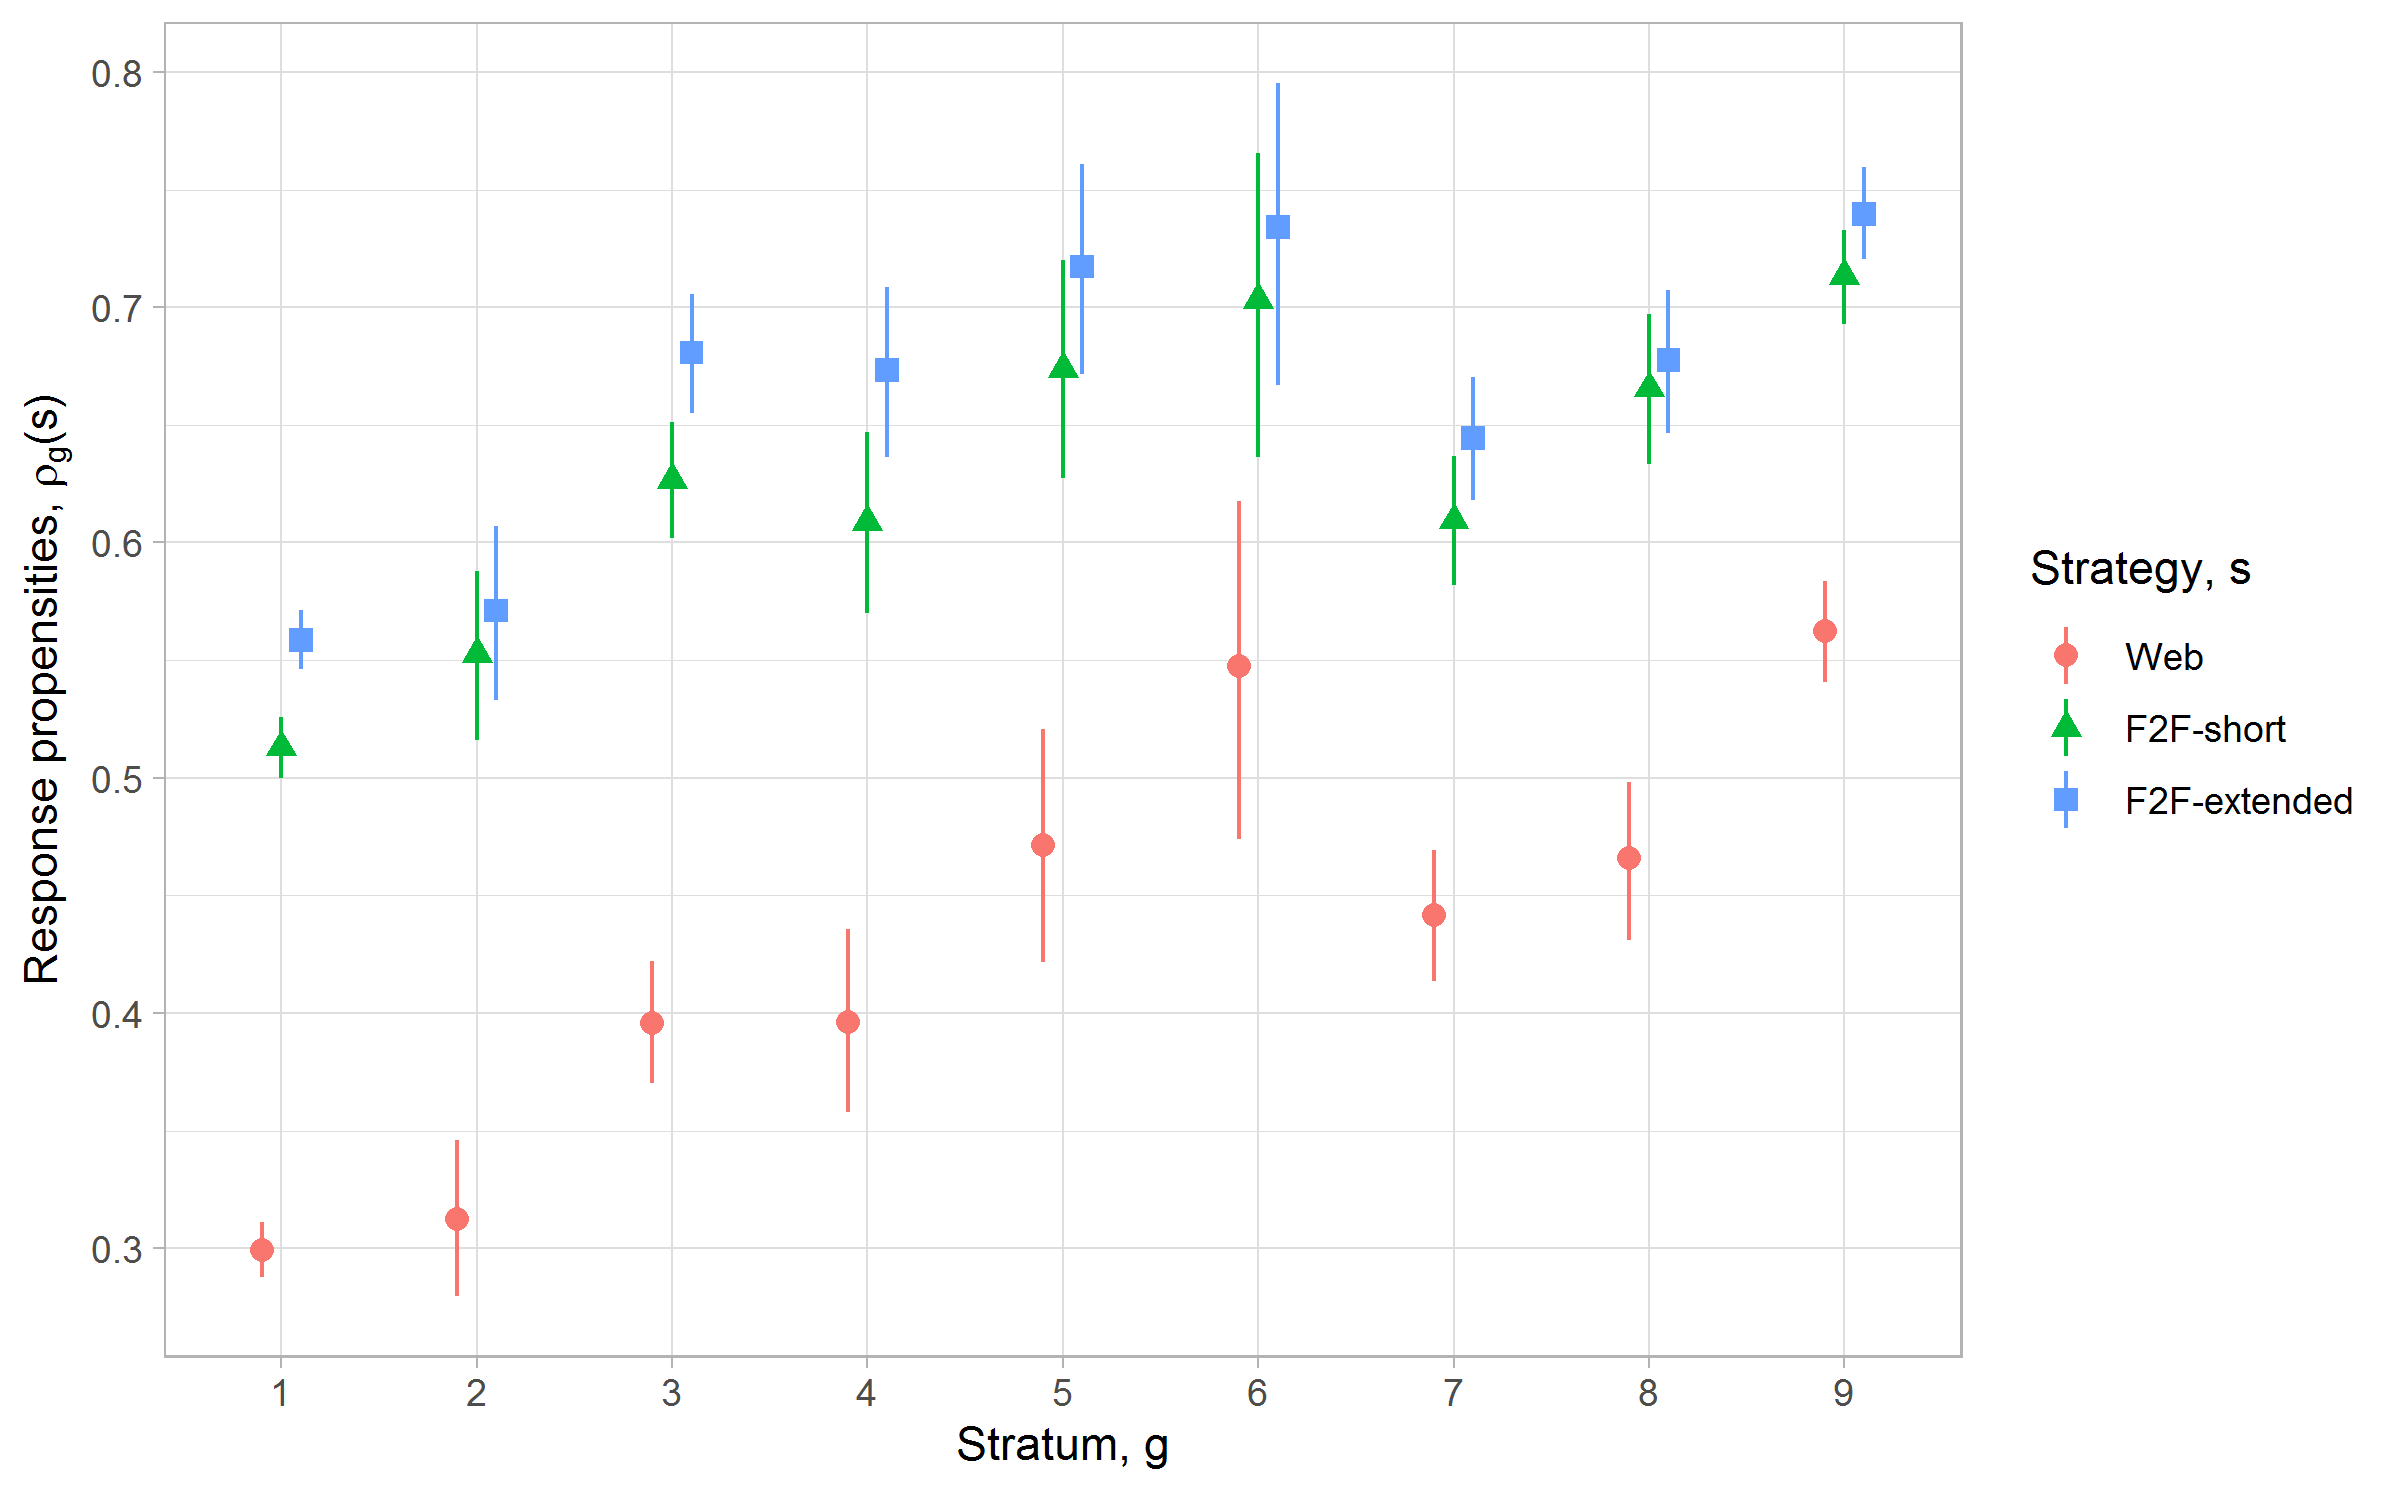
\includegraphics{images/propensitiesByStratum.png}}{}
\makeatother 
\caption{{Estimated Response Propensities per Stratum and Strategy.}}
\label{fig-strata-response-propensities}
\end{figure*}
\egroup

It is conspicuous that the variation in overall response propensities can be significant if a single strategy is implemented uniformly over the entire sample.
The optimization aims to find an optimal way to distribute different strategies among these unit groups, which will reduce the impact of nonresponse on the estimates of survey variables of interest.
Since the objective is to balance the responses, the estimates of costs per stratum and strategy are not shown to save space.


\subsection{Optimization, Optimal Stratification, and Optimal Adaptive Designs}
\label{subsec:optimization-optimal-stratification-optimal-adaptive-designs}

With the estimated response propensities and costs per stratum and strategy, the quality and cost indicators such as coefficient of variation of response propensities, response rate, and required budget per respondent can be derived to solve the optimization problem.
The application of the proposed and two other response- and cost-oriented stratification methods leads to three sets of solutions whose utility in balancing the responses with respect to the predicted survey variables will be assessed to determine the optimal stratification.
The adaptive survey design solutions based on such optimal stratification are regarded as the optimal solutions.

\subsubsection{Optimization problem}
\label{subsubsec:optimization-problem}

As a sample unit may receive one of the three strategies and can belong to one of the nine groups when the Response$\hat{Y}$ method is applied, the collection of survey designs, i.e., the allocations of strategies, $\mathcal{S}^9_{1,3}$, has a total of 19683 solutions.
Similarly, based on the ResponseX and CostX methods, the collections of survey designs have $\mathcal{S}^{10}_{1,3}=\text{59049}$ and $\mathcal{S}^7_{1,3}=\text{2187}$ solutions, respectively.
The optimization corresponds to selecting the optimal designs from a solution set such that the objective function of the coefficient of variation of response propensities is optimized subject to the constraints on the response rate and required budget per respondent.
For the Health Survey stakeholders, the lower limit of satisfactory response rate, $\mathrm{RR}_{\mathrm{lower}}$, is set at 50\%, and the upper limit of required budget per respondent, $\mathrm{B}_{\mathrm{upper}}$, is set at 42 EUR.
These conditions allow the filtering of the designs that satisfy the constraints, from which the objective function selects the designs with the minimal $\mathrm{CV}$.


\subsubsection{Optimal stratification}


Since it is not feasible to directly compare the optimization outputs based on different stratification methods, the top five optimal designs of each solution set are re-evaluated against the criterion developed in section \ref{subsec:determining-optimal-stratification}.
In the Bayesian analysis, non-informative priors are specified for the regression parameters of the stratification-assessed response propensity models.
The coefficients of variation of the response propensities for the fifteen design solutions are derived without the grouping structure, and their expectations are plotted along with the 95\% credible intervals in Figure \ref{fig-optimal-response-propensities}.
\bgroup
\fixFloatSize{images/CVcriterion.png}
\begin{figure*}[!htbp]
\centering \makeatletter\IfFileExists{images/CVcriterion.png}{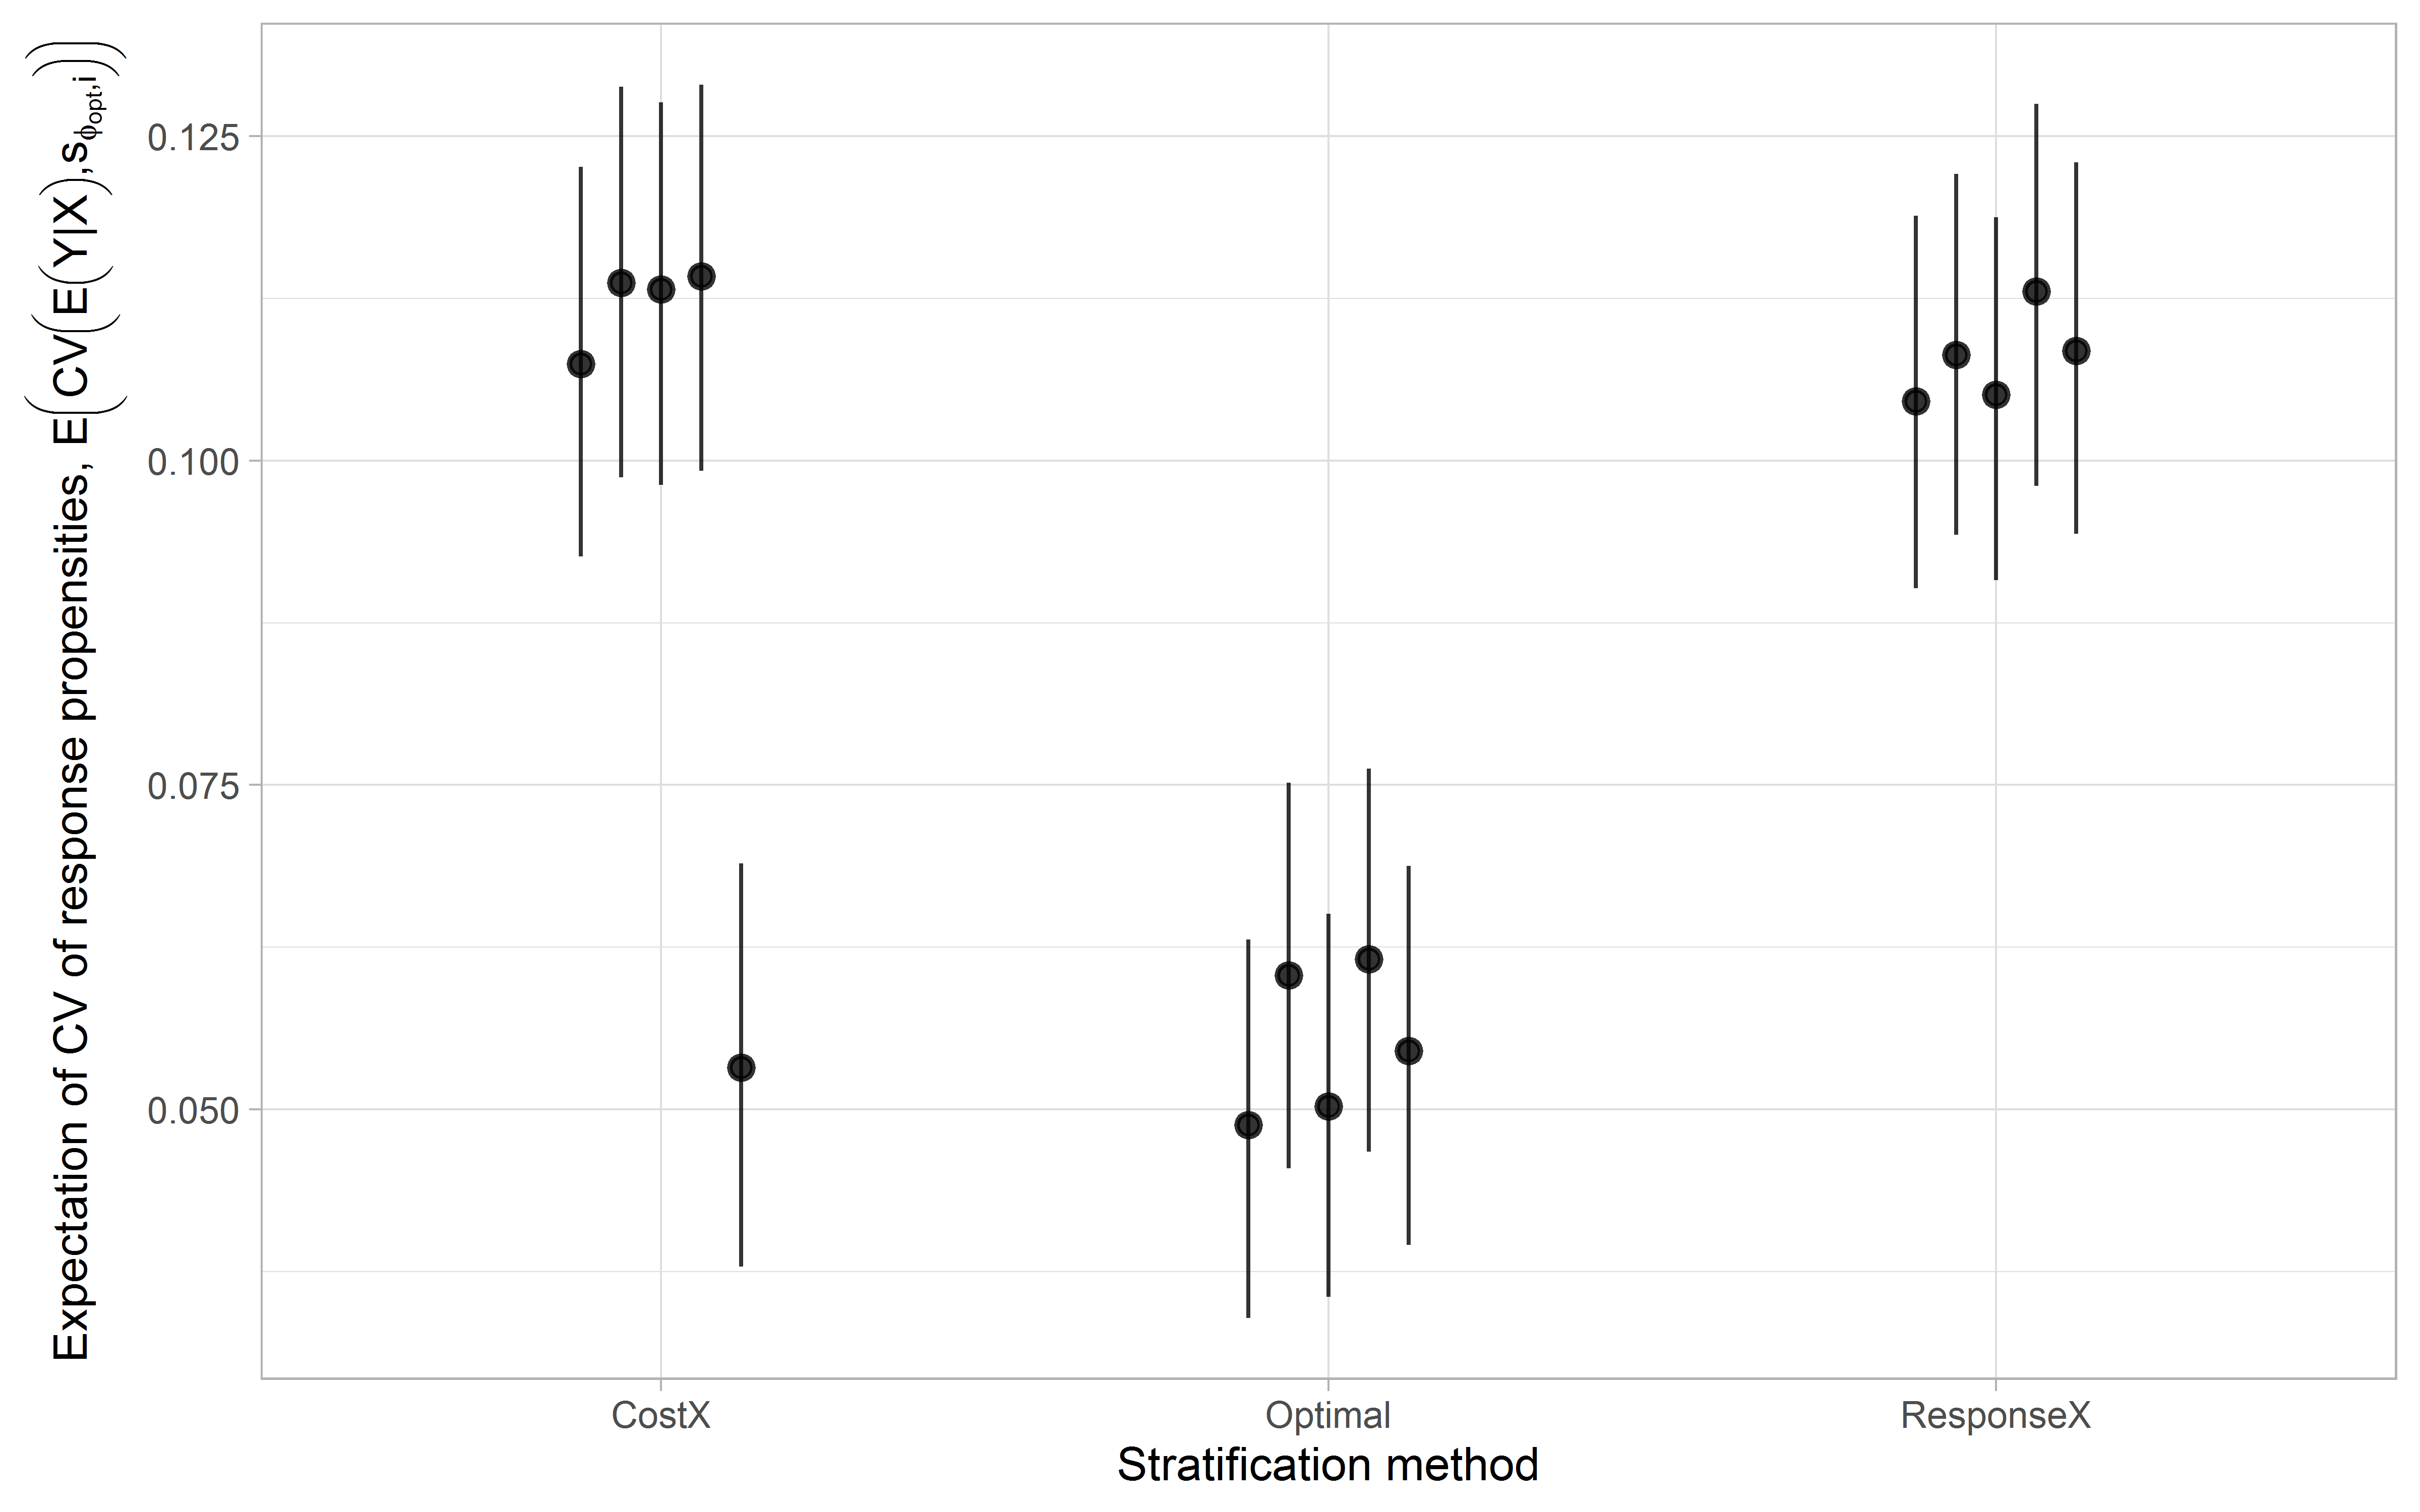
\includegraphics{images/CVcriterion.png}}{}
\makeatother 
\caption{{Expected Values of the Assessment Criterion, i.e., Coefficient of Variation (CV) of Response Propensities of Optimal Design Solutions Based on Different Stratification Methods.}}
\label{fig-optimal-response-propensities}
\end{figure*}
\egroup

It is shown that most optimal solutions selected based on the ResponseX and CostX methods tend to yield higher variation in response outcomes with respect to the predicted survey variables compared to those based on the proposed Response$\hat{Y}$ method.
Furthermore, there is no overlap in the 95\% credible intervals of the expectations of coefficient of variation between the Response$\hat{Y}$ method and others.
Only one solution based on the CostX method performs no less well.
In general, the proposed stratification method in this paper is superior to two other response- and cost-oriented methods in terms of minimizing the impact of nonresponse bias on the survey estimates of interest.

\subsubsection{Optimal adaptive survey designs}

To eventually address the optimization problem, Table \ref{tbl-optimal-designs} provides the strategy allocations as well as the expected values of the quality and cost indicators for the five optimal adaptive survey designs based on the optimal stratification method Response$\hat{Y}$.
\begin{sidewaystable*}[!htbp]
\caption{{Optimal Designs with Minimal Coefficient of Variation (CV) Subject to Constraints on Budget per Respondent (B) and Response Rate (RR).}}
\label{tbl-optimal-designs}
\def\arraystretch{1}
\ignorespaces 
\centering 
\begin{tabulary}{\linewidth}{LLLLLL}
\hline Stratum & Design 1 & Design 2 & Design 3 & Design 4 & Design 5\\
\hline 
1 & F2F-extended
   & F2F-extended
   & F2F-extended
   & F2F-extended
   & F2F-extended
  \\
2 & F2F-extended
   & F2F-extended
   & F2F-short
   & F2F-short
   & F2F-extended
  \\
3 & F2F-short
   & F2F-short
   & F2F-short
   & F2F-short
   & F2F-short
  \\
4 & F2F-short
   & F2F-short
   & F2F-short
   & F2F-short
   & F2F-short
  \\
5 & Web
   & F2F-short 
   & Web
   & F2F-short
   & Web
  \\
6 & Web
   & Web
   & Web
   & Web
   & F2F-short
  \\
7 & F2F-short
   & F2F-short
   & F2F-short
   & F2F-short
   & F2F-short
  \\
8 & Web
   & Web
   & Web
   & Web
   & Web
  \\
9 & Web
   & Web
   & Web
   & Web
   & Web
  \\
\hline\hline
$\mathbb{E}\left(\mathrm{CV}\right)$ & \makecell{ 0.0727 \\ [-1ex] (0.0584, 0.0874) }
  & \makecell{ 0.0729 \\ [-1ex] (0.0587, 0.0869) }
  & \makecell{ 0.0730 \\ [-1ex] (0.0589, 0.0876) }
  & \makecell{ 0.0734 \\ [-1ex] (0.0592, 0.0873) }
  & \makecell{ 0.0777 \\ [-1ex] (0.0636, 0.0923) }
  \\
$\mathbb{E}\left(\mathrm{B}\right)$ & \makecell{ 40.16 \\ [-1ex] (39.07, 41.26) }
  & \makecell{ 41.08 \\ [-1ex] (39.98, 42.20) }
  & \makecell{ 40.03 \\ [-1ex] (38.94, 41.13) }
  & \makecell{ 40.95 \\ [-1ex] (39.85, 42.08) }
  & \makecell{ 40.52 \\ [-1ex] (39.43, 41.63) }  
  \\
$\mathbb{E}\left(\mathrm{RR}\right)$ & \makecell{ 56.6\% \\ [-1ex] (0.557, 0.574) }
  & \makecell{ 57.1\% \\ [-1ex] (0.563, 0.580) }
  & \makecell{ 56.5\% \\ [-1ex] (0.556, 0.573) }
  & \makecell{ 57.0\% \\ [-1ex] (0.562, 0.579) }
  & \makecell{ 56.8\% \\ [-1ex] (0.560, 0.576) }
  \\
\hline
\multicolumn{6}{l}{\textit{Note:} 95\% Credible intervals in parentheses.}
\end{tabulary}\par 
\end{sidewaystable*}

Meanwhile, it is important to emphasize that under the Bayesian analysis, the objective function and constraints are random, which means that no single design solution is superior, but rather there is a range of solutions with similar performance.
In Figure \ref{fig-optimal-designs}, for the top 150 design solutions, their expectations of coefficient of variation of the response propensities are plotted against the expectations of budget per respondent and response rate.
While the top five solutions stand out, their 95\% credible intervals of coefficient of variation still partially overlap with those of a range of solutions.
Some of these solutions also yield similar budgets per respondent and response rates.
Overall, this figure illustrates the uncertainty of the optimal designs and suggests the need for further research on the sensitivity of the optimal designs.
%Health Survey stakeholders can implement one of the optimal designs in the future round of the survey.
%These four optimal allocations of strategies and their expected values of the quality and cost indicators are shown in Table \ref{tbl-optimal-designs}.
\bgroup
%\fixFloatSize{images/optimalCVvB.png}
\begin{figure*}[!htbp]
\centering \makeatletter
\begin{subfigure}{.5\textwidth}
	\centering
	\IfFileExists{images/optimalCVvB.png}{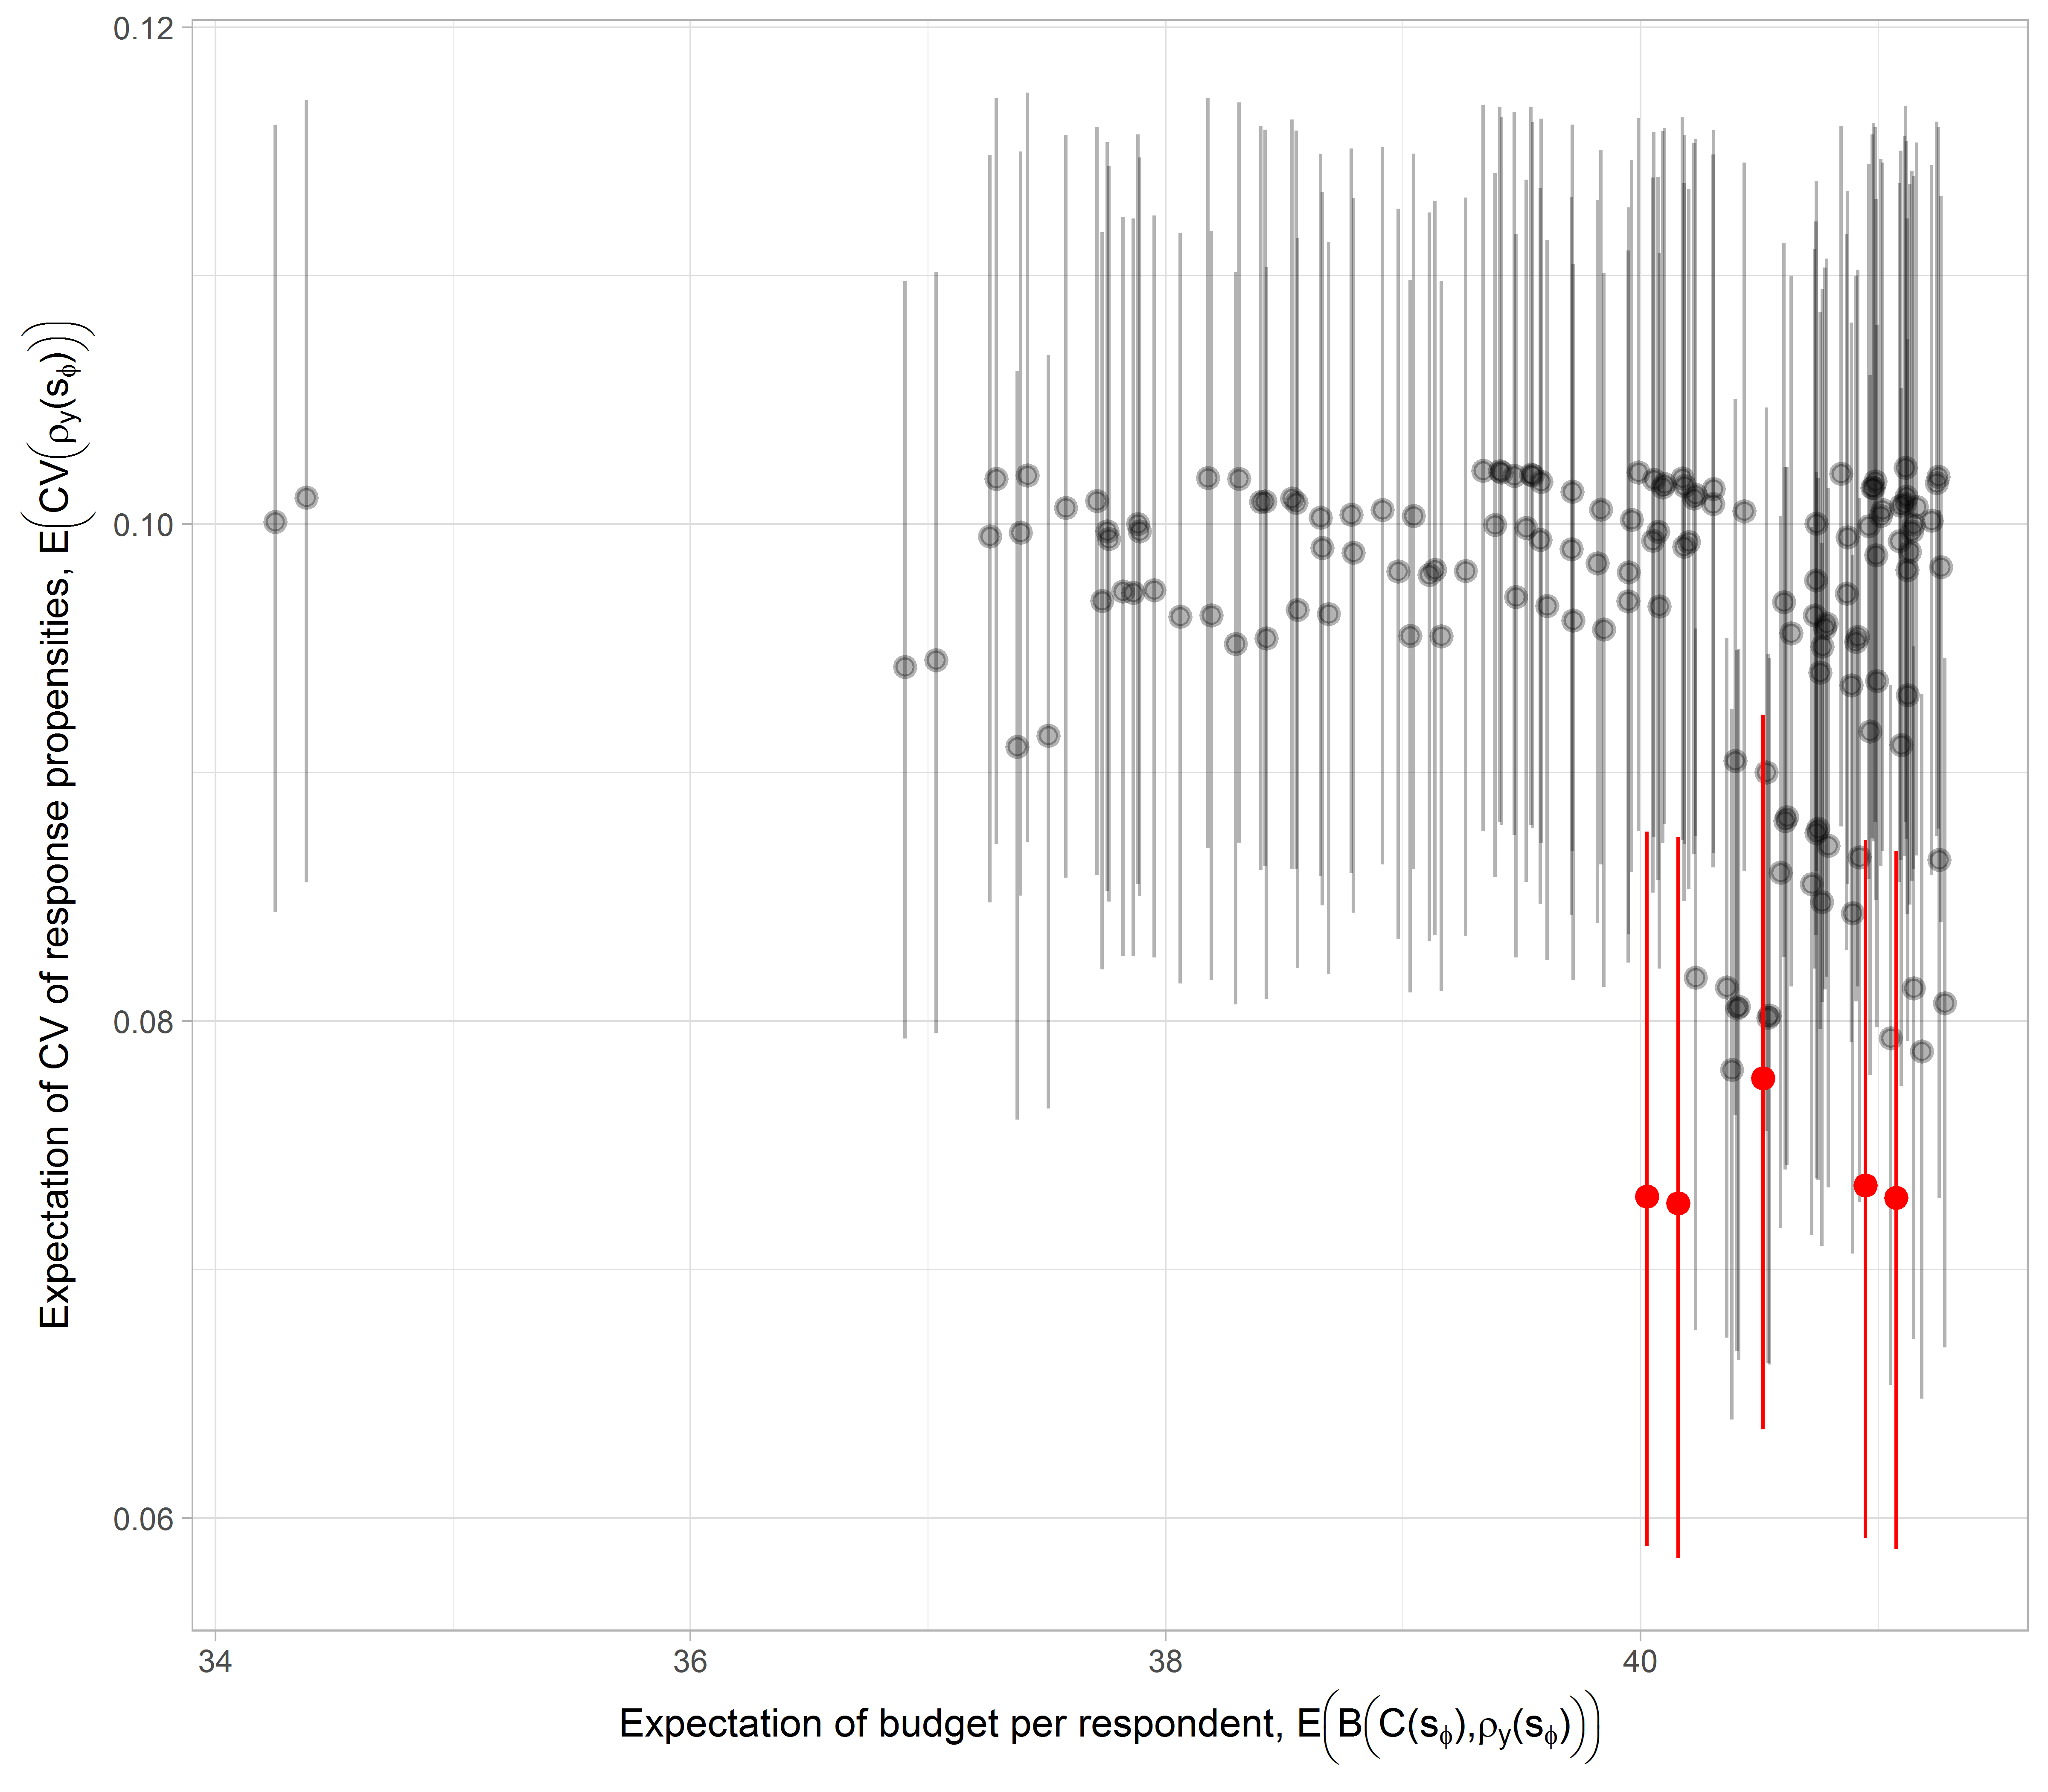
\includegraphics{images/optimalCVvB.png}}{}
\end{subfigure}%
\begin{subfigure}{.5\textwidth}
	\centering
	\IfFileExists{images/optimalCVvRR.png}{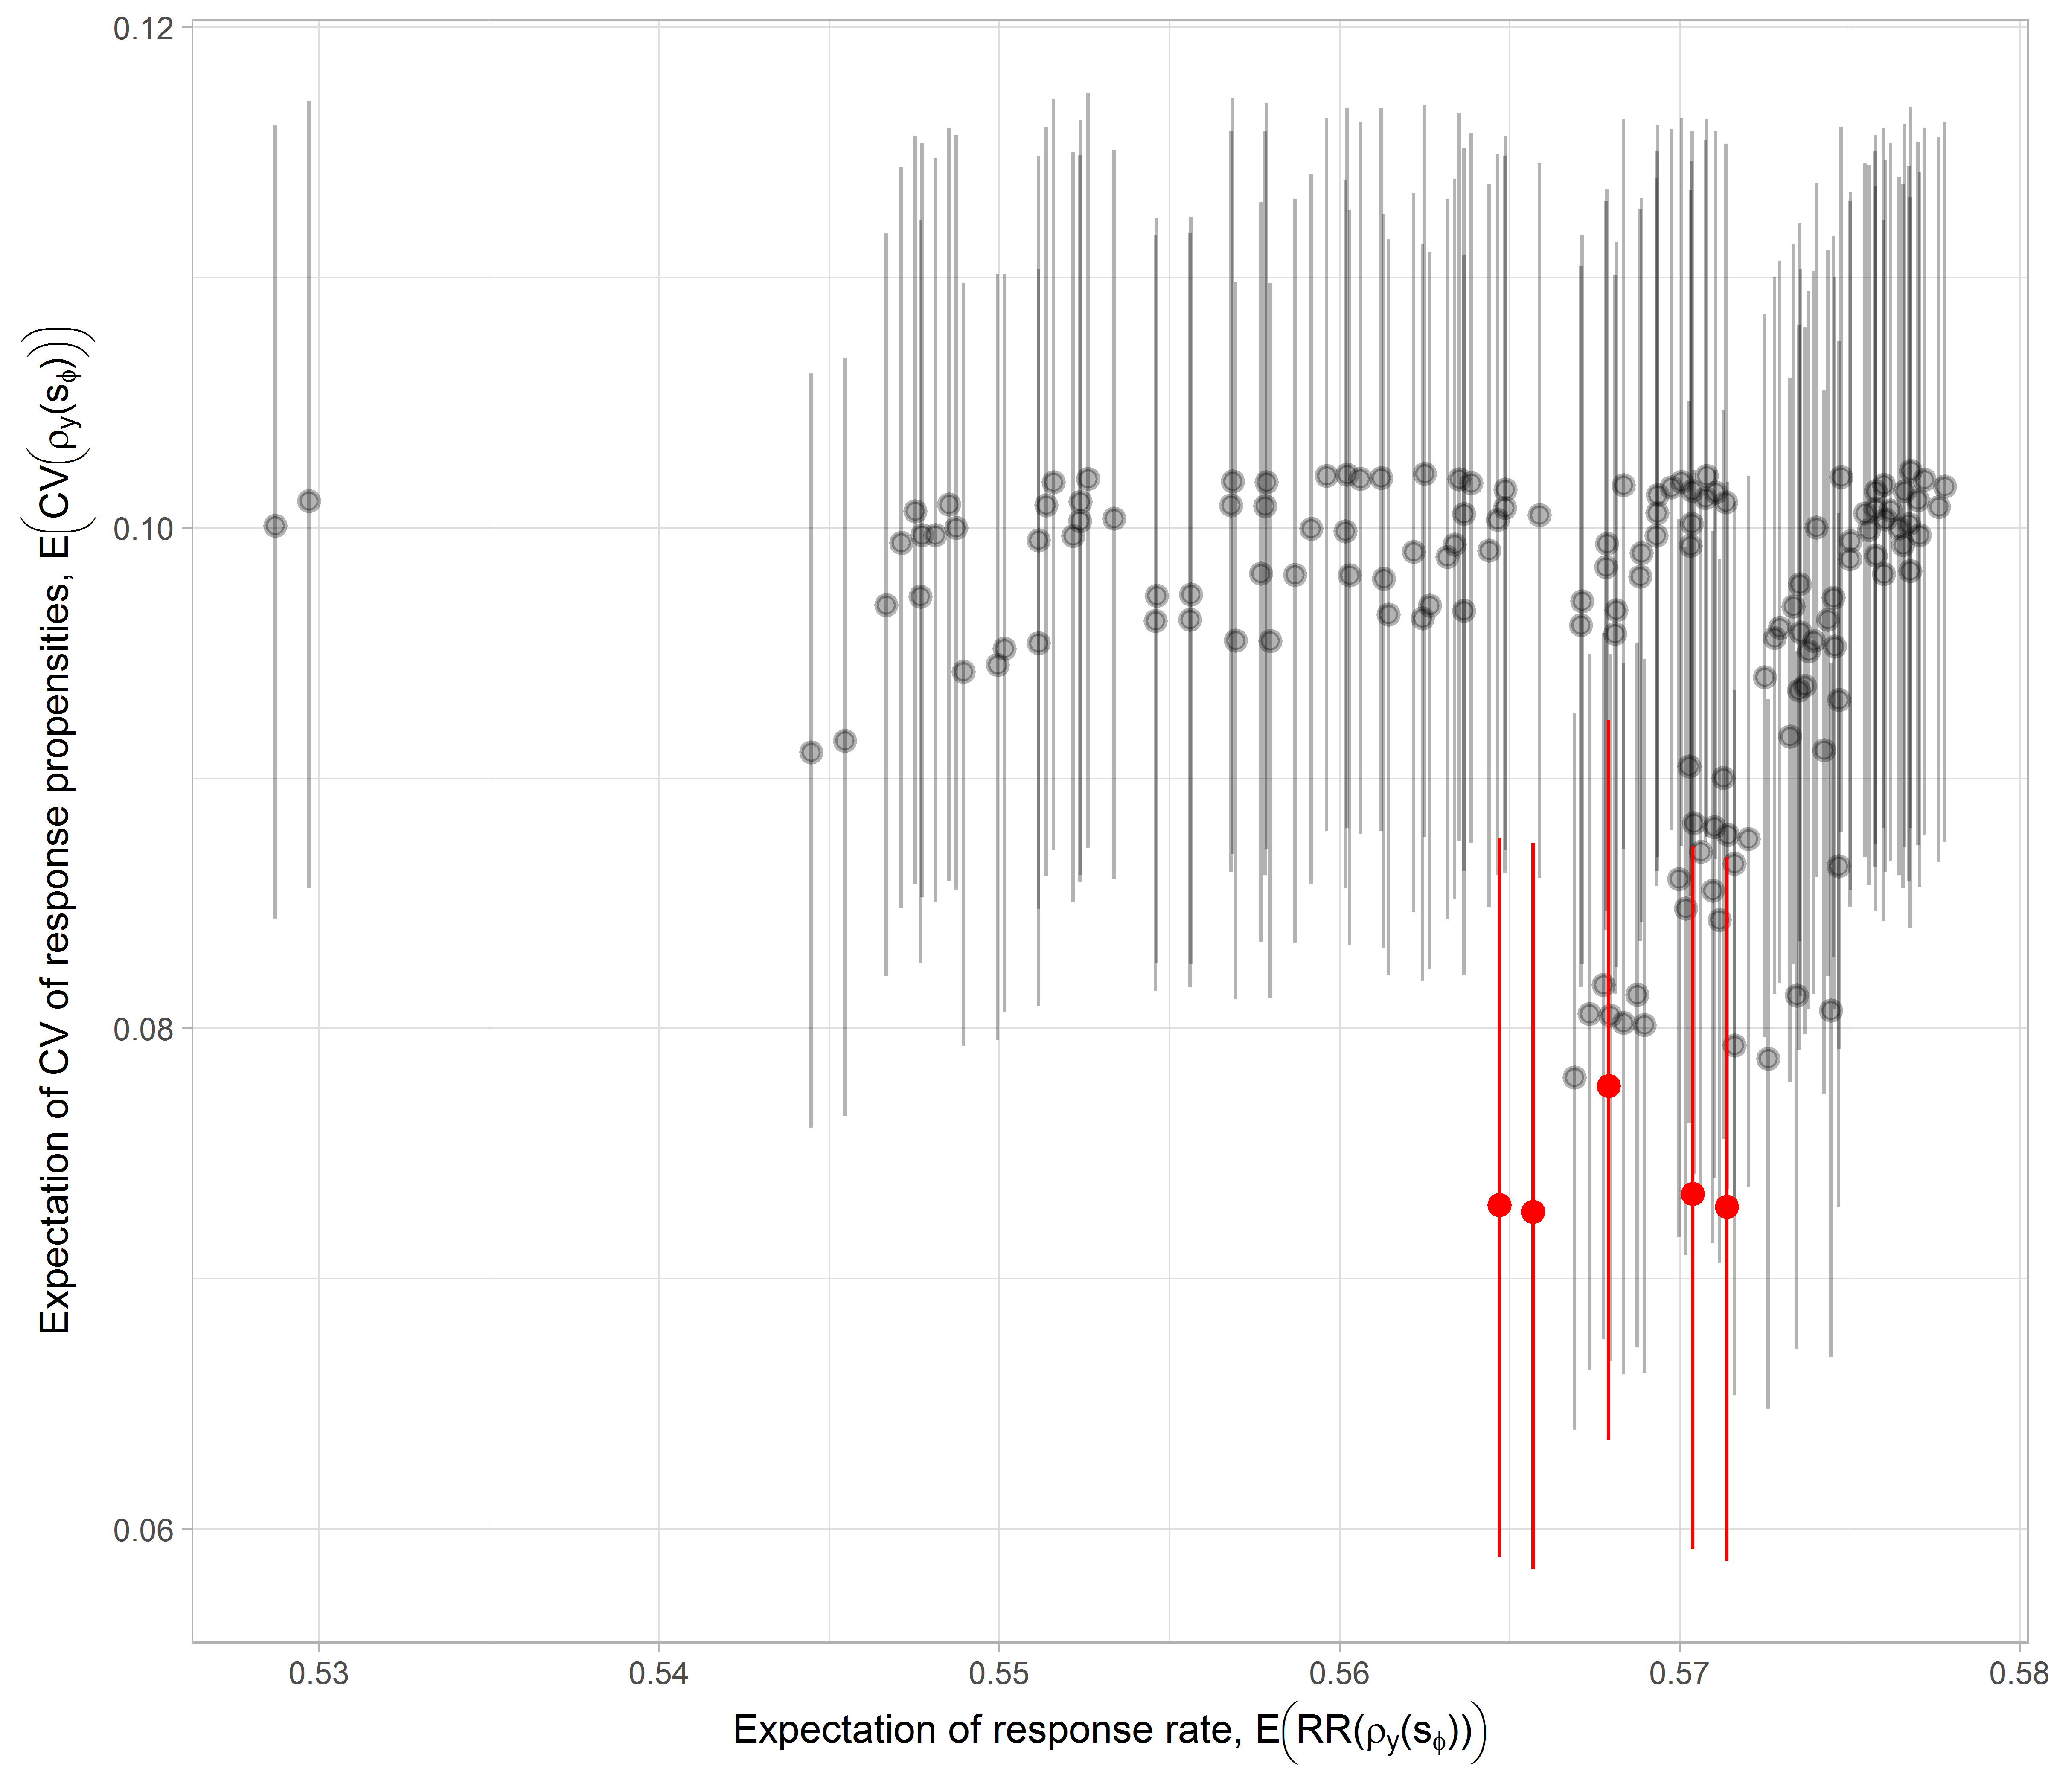
\includegraphics{images/optimalCVvRR.png}}{}
\end{subfigure}%
\makeatother
\caption{{Expected Values of Coefficient of Variation (CV) of Response Propensities of Top 150 Design Solutions Satisfying the Constraints on Budget per Respondent (B) and Response Rate (RR). Top 5 Optimal Solutions Marked in Red.}}
\label{fig-optimal-designs}
\end{figure*}
\egroup

%Starting from the fifth optimal solution, the expected value of $\mathrm{CV}$ is gradually higher than the top four.
%Obviously, a high response rate means more time and money invested, but it does not necessarily mean lower variation in response outcomes.




%\subsection{Evaluation of Optimal Designs Based on Different Stratification}
%\label{comparison-optimal-designs-different-stratification}

%The optimal designs should produce as little variation in response outcomes as possible.
%To demonstrate the optimal designs shown above achieving this objective better than those based on other stratification, this case study also applies two other stratification methods to solve the same optimization problem and evaluates their outputs against the same criterion.
%One common method (ResponseX) is to use the auxiliary data directly as input to the classification tree algorithm to account for differences in responses to web mode, which does not involve the survey variables of interest.
%Another method (CostX) targets the detection of heterogeneity in survey costs, which is used for the objective of minimizing the budget rather than the variation in response outcomes.
%This method also takes the auxiliary data as input, and produces clusters of units that differ most in cost related variables such as the number of in-person visits.

%Applying both stratification methods to the same data, the former one yields ten strata and with the latter, seven strata.
%which means that based on these two stratification schemes, the feasible regions of the optimization problem, i.e., the collections of designs have 59049 and 2187 solutions, respectively.
%After solving the optimization problem, the top five solutions are selected from each of the two collections.

%To evaluate three sets of optimal designs based on different stratification schemes, I reassign the observed response outcomes accordingly to mimic the response results in the case of implementing the optimal designs.
%Based on the reconstructed responses, the individual response propensities are estimated by the expectations of survey variables.


    
\section{Discussion}
\label{sec:discussion}


This paper answers the main research question by implementing an optimal approach to stratify the target population into subgroups and demonstrating its effectiveness and efficiency through a coefficient of variation criterion after the optimization of adaptive survey designs.
The optimal adaptive survey designs constructed based on such stratification method perform robustly and minimizes nonresponse bias compared to the other two response- and cost-oriented stratification methods.

The entire process of conducting adaptive survey designs needs to be presented, including generating subgroups, estimating the survey design parameters such as response propensity and cost for each subgroup under each data collection strategy, and optimally filtering out the optimal design solutions, i.e., the optimal allocations of strategies to subgroups, subject to a number of specified constraints.

The optimal stratification method is implemented to generate subgroups based on predicted survey variables.
Prior to stratification, this method entails predicting unobserved survey variables with available auxiliary data before data collection starts.
Assisted by a wealth of administrative data, many multi-phase, mixed-strategy surveys conducted by statistical institutes can employ this method.
To minimize the impact of nonresponse on survey estimates, this method makes it possible to balance responses in subgroups consisting of ranges of predicted values or probabilities for the survey variables.
Theoretically, optimized allocations of the data collection strategies to such subgroups would produce minimal response variation with respect to the survey variables.
This paper accordingly develops a coefficient of variation criterion to quantify the utility of this method compared to other stratification methods that do not involve survey variables.
The comparison is illustrated by a case study optimizing adaptive survey designs based on this novel stratification method and two other response- and cost-oriented methods.
The case study shows that the optimal design solutions based on this novel stratification method yield less variation in response behavior with respect to the predicted survey variables.

The analysis performed in this paper is based on a Bayesian framework, except for the classification tree algorithm.
The predicted survey variables take the expected values of their posterior predictive distributions given the model parameters repeatedly drawn in a Gibbs sampler.
The classification algorithm takes the predicted survey variables as inputs and outputs several subgroups.
Optimization is performed to search for the optimal allocations of the data collection strategies to these subgroups by comparing the quality indicators, such as the response rate or coefficient of variation of response propensities, and cost indicators.
Since the quality and cost indicators are functions of the response propensities and costs, their posterior distributions can be derived as important by-products of the posterior distributions of the response propensities and costs whose estimates are provided by a Gibbs sampler.
The posterior distribution of the coefficient of variation criterion for determining the optimal stratification is also derived in a similar manner.

It is to be emphasized that when solving the optimization problem under Bayesian analysis, the optimal design solutions are selected based on artificial posterior distributions of the quality and cost indicators.
Since the size of a solution set grows exponentially when the number of subgroups increases, it is computationally laborious to derive the posterior distributions of the quality and cost indicators for every design solution by evaluating the corresponding response propensity and cost models.
A more elegant optimization approach remains to be developed, which is not the focus of this paper.
The alternative optimization approach adopted in this paper is sufficient to output the optimal design solutions for the assessment of different stratification methods.

The novel stratification method excels in reducing nonresponse bias in survey estimates because it relies on the predicted survey variables to stratify, which means that this method is limited by the predictive power of the available auxiliary data for key survey variables.
In an extreme case, there could be no available auxiliary variables that are predictors of the survey variables.
It warrants sensitivity analyses and simulation studies in future research to examine the impact of inaccurate survey variable predictions on this stratification method.
Moreover, this paper does not consider the strategy-dependent measurement error of the survey variables, which may impinge on the accuracy of predicted survey variables.
Such an extension is worthwhile for mixed-mode survey design and is subject to future research.

This paper demonstrates the advantages of this novel stratification method over two other response- and cost-oriented methods, but space does not permit the assessment of more existing methods such as partial representativeness indicators and regression diagnostic measures\unskip~\cite{Schouten:2017:isr,Wagner:2014}.
With the assessment criterion developed by this paper, however, future studies can specifically assess all the different stratification methods.

Ultimately, the optimal stratification allows parsimonious use of auxiliary information to account for heterogeneity in both response behavior and key survey variables.
Such an application implies that the optimal allocations of strategies to the resulting strata should have enhanced capacity to reduce nonresponse bias effectively and efficiently.

%A subsequent Bayesian analysis of response propensities is a requisite for further analysis of quality indicators and optimization of adaptive designs. 
%To implement a complete process of selecting optimal designs, several elements should be added to this paper. 
%The limited budget to conduct a survey requires the analysis of cost parameters in each step of data collection. 
%By setting constraints on the total cost, the optimal designs are subjected to the required budget. 
%Besides, to be able to incorporate dynamic adaptive survey designs, paradata obtained during data collection may also be included in the response propensity models.
%While building Bayesian models, it is crucial to elicit prior knowledge from an appropriate amount of historic survey data.

%After the optimization of adaptive designs, future research can further demonstrate the strengths and limitations of this stratification method.
%This method relies on the predictive power of auxiliary variables to the target survey variables, which varies in different surveys. 
%In the case study, this method can perform well as the predictions on the Health Survey variables are satisfactory.
%The advantages can be substantiated by applying other methods in the Health Survey and comparing their performance with this method.
%However, in an extreme case, there could be no available auxiliary variables that are predictors of the survey variables.
%The utility of this method in reducing nonresponse bias might not outstrip other methods. More surveys should be involved to examine the applicability and corresponding conditions of this new method. 




\clearpage
\appendix

\counterwithin{figure}{section}
\counterwithin{table}{section}

\begin{appendices}
\section{Full Conditionals}
\label{appendix-full-conditionals}

This appendix contains expressions for the full conditionals of the regression model parameters for survey variables, response propensities, and costs that are sampled in the Gibbs sampler.

\subsection{Full conditionals for regression parameters of dichotomous variable models}
\label{appendix-full-conditionals-dichotomous-variables}

Models for dichotomous survey variables and response propensities have the following general form:
\let\saveeqnno\theequation
\let\savefrac\frac
\def\dispfrac{\displaystyle\savefrac}
\begin{eqnarray*}
\let\frac\dispfrac
%\gdef\theequation{}
\let\theHequation\theequation
%\label{}
%\begin{array}{@{}l}
	Z_{D,i}=\Theta_{D}X_{D,i}+\varepsilon_{D,i},
%\end{array}
\end{eqnarray*}
\global\let\theequation\saveeqnno
\addtocounter{equation}{-1}\ignorespaces

where $D$ represents one of three probit models (\ref{equation-dichotomous-survey-variables}), (\ref{equation-latent-response}), and (\ref{equation-latent-optimal}), for one of which $Z_{D,i}$ is a latent variable, and $X_{D,i}$ is a column vector of covariates, and the regression parameters are the slope parameters in the vector $\Theta_D$.
The latent variable $Z_{D,i}$, which is not of direct interest, is updated in the Gibbs sampler to derive the probability of success.
Although three models have different outcomes and predictors, it is analogous for the derivation of full conditionals.

For the slope paramter $\Theta_D \in \{\theta_D,\alpha_{s_{\phi_{\mathrm{opt}}}}\}$, the prior distribution is normal $\Theta_D \sim \mathcal{N}\left(\mu_{\Theta_D},\Sigma_{\Theta_D}\right)$.
The full conditional distribution is also normal, denoted as,
\let\saveeqnno\theequation
\let\savefrac\frac
\def\dispfrac{\displaystyle\savefrac}
\begin{eqnarray}
\let\frac\dispfrac
\gdef\theequation{A1}
\let\theHequation\theequation
\label{equation-full-conditionals-dichotomous}
%\begin{array}{@{}l}
	(\Theta_{D}|u_D,Z_D,X_D) \sim \mathcal{N}(\mu_{FULL,D},\Sigma_{FULL,D}).
%\end{array}
\end{eqnarray}
\global\let\theequation\saveeqnno
\addtocounter{equation}{-1}\ignorespaces

The expectation and covariance of the full conditional distribution for a model are derived as follows:
\let\saveeqnno\theequation
\let\savefrac\frac
\def\dispfrac{\displaystyle\savefrac}
\begin{eqnarray}
\let\frac\dispfrac
\gdef\theequation{A2}
\let\theHequation\theequation
\label{equation-full-conditionals-dichotomous-sigma}
%\begin{array}{@{}l}
	\Sigma_{FULL,D}=\left(\Sigma^{-1}_{\Theta_D}+X_D^TX_D\right)^{-1},
%\end{array}
\end{eqnarray}
\begin{eqnarray}
\let\frac\dispfrac
\gdef\theequation{A3}
\let\theHequation\theequation
\label{equation-full-conditionals-dichotomous-mu}
%\begin{array}{@{}l}
	\mu_{FULL,D}=\Sigma_{FULL,D}\left(\Sigma^{-1}_{\Theta_D}\mu_{\Theta_D}+X_D^TZ_D\right).
%\end{array}
\end{eqnarray}
\global\let\theequation\saveeqnno
\addtocounter{equation}{-1}\ignorespaces

The latent variable follows the truncated normal distribution, $(Z_{D,i}|\Theta_D,X_D) \sim \mathcal{TN}(\Theta_DX_{D,i},1)$.
When the outcome $u_{D,i}=1$, then $Z_{D,i}>0$ and $(Z_{D,i}|u_{D},\Theta_D,X_D)$ is the normal distribution restricted to the positive real axis.
For $u_{D,i}=0$, $(Z_{D,i}|u_{D},\Theta_D,X_D)$ is the normal distribution restricted to the non-positive real axis.


\subsection{Full conditionals for regression parameters of continuous variable models}
\label{appendix-full-conditionals-continuous-variables}

For continuous survey variable and cost models, the derivation of full conditionals is analogous. The model has the following general form:
\let\saveeqnno\theequation
\let\savefrac\frac
\def\dispfrac{\displaystyle\savefrac}
\begin{eqnarray*}
\let\frac\dispfrac
%\gdef\theequation{}
\let\theHequation\theequation
%\label{}
%\begin{array}{@{}l}
	Y_{C,i}=\theta_{C}X_{C,i}+\varepsilon_{C,i},
%\end{array}
\end{eqnarray*}
\begin{eqnarray*}
\let\frac\dispfrac
%\gdef\theequation{}
\let\theHequation\theequation
%\label{}
%\begin{array}{@{}l}
	\varepsilon_{C,i} \sim \mathcal{N}(0,\zeta),
%\end{array}
\end{eqnarray*}
\global\let\theequation\saveeqnno
\addtocounter{equation}{-1}\ignorespaces

where $C$ represents one of two linear models (\ref{equation-continuous-survey-variables}) and (\ref{equation-cost}), for one of which $Y_{C,i}$ is either the continuous survey variable or the realized costs, and $X_{C,i}$ is a column vector of covariates, and $\varepsilon_{C,i}$ is phase-dependent error term. In this paper, the costs depend on the phase but not on the action itself.
The regression slope parameters $\theta_C$ and the dispersion parameters $\zeta$ need to be updated.

For the slope parameter $\theta_C$, the prior distribution is normal $\theta_C \sim \mathcal{N}\left(\mu_{\theta_C},\Sigma_{\theta_C}\right)$.
The full conditional distribution is also normal, denoted as,
\let\saveeqnno\theequation
\let\savefrac\frac
\def\dispfrac{\displaystyle\savefrac}
\begin{eqnarray}
\let\frac\dispfrac
\gdef\theequation{A4}
\let\theHequation\theequation
\label{equation-full-conditionals-continuous-slope}
%\begin{array}{@{}l}
	(\theta_{C}|Y_C,X_C,\zeta) \sim \mathcal{N}(\mu_{FULL,C},\Sigma_{FULL,C}).
%\end{array}
\end{eqnarray}
\global\let\theequation\saveeqnno
\addtocounter{equation}{-1}\ignorespaces

The expectation and covariance of the full conditional distribution for a model are derived as follows:
\let\saveeqnno\theequation
\let\savefrac\frac
\def\dispfrac{\displaystyle\savefrac}
\begin{eqnarray}
\let\frac\dispfrac
\gdef\theequation{A5}
\let\theHequation\theequation
\label{equation-full-conditionals-continuous-sigma}
%\begin{array}{@{}l}
	\Sigma_{FULL,C}=\left(\dfrac{1}{\zeta}X_C^TX_C+\left(\Sigma^2_{\theta_C}\right)^{-1}\right)^{-1},
%\end{array}
\end{eqnarray}
\begin{eqnarray}
\let\frac\dispfrac
\gdef\theequation{A6}
\let\theHequation\theequation
\label{equation-full-conditionals-continuous-mu}
%\begin{array}{@{}l}
	\mu_{FULL,C}=\Sigma_{FULL,C}\left(\dfrac{1}{\zeta}X_C^TY_C+\left(\Sigma^2_{\theta_C}\right)^{-1}\mu_{\theta_C}\right).
%\end{array}
\end{eqnarray}
\global\let\theequation\saveeqnno
\addtocounter{equation}{-1}\ignorespaces

For the dispersion parameter $\zeta$, the prior distribution is inverse Gamma $\zeta \sim \Gamma^{-1}(a_\zeta,b_\zeta)$. The full conditional is also inverse Gamma:
\let\saveeqnno\theequation
\let\savefrac\frac
\def\dispfrac{\displaystyle\savefrac}
\begin{eqnarray}
\let\frac\dispfrac
\gdef\theequation{A7}
\let\theHequation\theequation
\label{equation-full-conditionals-continuous-dispersion}
%\begin{array}{@{}l}
	(\zeta|\theta_C,Y_C,X_C) \sim \Gamma^{-1}(a_{FULL},b_{FULL}),
%\end{array}
\end{eqnarray}
\global\let\theequation\saveeqnno
\addtocounter{equation}{-1}\ignorespaces

where the hyperparameters are derived as follows:
\let\saveeqnno\theequation
\let\savefrac\frac
\def\dispfrac{\displaystyle\savefrac}
\begin{eqnarray}
\let\frac\dispfrac
\gdef\theequation{A8}
\let\theHequation\theequation
\label{equation-full-conditionals-continuous-a}
%\begin{array}{@{}l}
	a_{FULL}=a_{\zeta}+\dfrac{n}{2},
%\end{array}
\end{eqnarray}
\begin{eqnarray}
\let\frac\dispfrac
\gdef\theequation{A9}
\let\theHequation\theequation
\label{equation-full-conditionals-continuous-b}
%\begin{array}{@{}l}
	b_{FULL}=b_{\zeta}+\dfrac{1}{2}\left(Y_C-X_C\theta_C\right)^T\left(Y_C-X_C\theta_C\right).
%\end{array}
\end{eqnarray}
\global\let\theequation\saveeqnno
\addtocounter{equation}{-1}\ignorespaces



\section{Results of Survey Variable Models}
\label{appendix-results-survey-variable-models}

The following table shows the results of modeling three dichotomized survey variables which are general health, smoking, and obesity.
The auxiliary data provides nine categorical predictors, including age, sex, income, marital status, level of education, migration background, receiving rent benefit, type of household, urbanization level of the area of residence.
Not all of them are predictors of the survey variables.
The best performing model for each survey variable is selected based on the deviance information criterion\unskip~\cite{Spiegelhalter:2002}.
The model fit is quantified by Bayesian $R^2$\unskip~\cite{Gelman:2019}.
\begin{longtable}{lccc}
    \caption{Probit Models of Survey Variables Predicted by Auxiliary Data.} \\
    \hline
     & General Health & Smoking & Obesity \\
    \hline
    \endfirsthead

    \multicolumn{4}{c}
    {\tablename\ \thetable{:} Probit Models of Survey Variables Predicted by Auxiliary Data (continued).} \\
    \hline
     & General Health & Smoking & Obesity \\ 
    \hline
    \endhead
    
    \hline \multicolumn{4}{r}{{(to be continued)}} \\
    \endfoot
    
    \endlastfoot
    
    Age (12--17) & & & \\  
    ~~~~18--24 & \makecell{ -0.172 \\ [-1ex] (-0.407, 0.069) } 
               & \makecell{ 0.955 \\ [-1ex] (0.722, 1.192) }
               & \makecell{ 0.270 \\ [-1ex] (-0.059, 0.599) } \\ 
    ~~~~25--29 & \makecell{ -0.417 \\ [-1ex] (-0.681, -0.161) }
               & \makecell{ 1.125 \\ [-1ex] (0.857, 1.383) }
               & \makecell{ 1.009 \\ [-1ex] (0.685, 1.314) } \\ 
    ~~~~30--34 & \makecell{ -0.575 \\ [-1ex] (-0.842, -0.301) }
               & \makecell{ 1.274 \\ [-1ex] (1.009, 1.534) }
               & \makecell{ 1.119 \\ [-1ex] (0.797, 1.449) } \\ 
    ~~~~35--39 & \makecell{ -0.700 \\ [-1ex] (-0.966, -0.426) }
               & \makecell{ 1.209 \\ [-1ex] (0.950, 1.468) }
               & \makecell{ 1.253 \\ [-1ex] (0.931, 1.560) } \\ 
    ~~~~40--44 & \makecell{ -0.855 \\ [-1ex] (-1.118, -0.593) }
               & \makecell{ 1.265 \\ [-1ex] (1.000, 1.529) }
               & \makecell{ 1.261 \\ [-1ex] (0.952, 1.576) } \\ 
    ~~~~45--49 & \makecell{ -1.049 \\ [-1ex] (-1.311, -0.794) }
               & \makecell{ 1.123 \\ [-1ex] (0.862, 1.379) }
               & \makecell{ 1.286 \\ [-1ex] (0.987, 1.586) } \\ 
    ~~~~50--54 & \makecell{ -1.074 \\ [-1ex] (-1.327, -0.812) }
               & \makecell{ 1.064 \\ [-1ex] (0.804, 1.329) }
               & \makecell{ 1.308 \\ [-1ex] (1.005, 1.606) } \\ 
    ~~~~55--59 & \makecell{ -1.251 \\ [-1ex] (-1.509, -0.992) }
               & \makecell{ 0.976 \\ [-1ex] (0.709, 1.243) }
               & \makecell{ 1.356 \\ [-1ex] (1.063, 1.655) } \\ 
    ~~~~60--64 & \makecell{ -1.460 \\ [-1ex] (-1.723, -1.191) }
               & \makecell{ 0.941 \\ [-1ex] (0.681, 1.208) }
               & \makecell{ 1.313 \\ [-1ex] (1.019, 1.609) } \\ 
    ~~~~65--69 & \makecell{ -1.221 \\ [-1ex] (-1.492, -0.943) }
               & \makecell{ 0.677 \\ [-1ex] (0.396, 0.953) }
               & \makecell{ 1.365 \\ [-1ex] (1.067, 1.666) } \\ 
    ~~~~$\geq$ 70 & \makecell{ -1.416 \\ [-1ex] (-1.683, -1.149) }
                  & \makecell{ 0.460 \\ [-1ex] (0.186, 0.736) }
                  & \makecell{ 1.213 \\ [-1ex] (0.920, 1.509) } \\ 
    Female (Male) & \makecell{ -0.056 \\ [-1ex] (-0.127, 0.014) }
                  & \makecell{ -0.294 \\ [-1ex] (-0.366, -0.222) }
                  &  \\ 
    Income (Missing) & & & \\
    ~~~~0--20\% perc & \makecell{ -0.061 \\ [-1ex] (-0.213, 0.089) }
                     & \makecell{ 0.213 \\ [-1ex] (0.056, 0.372) }
                     & \makecell{ 0.108 \\ [-1ex] (-0.063, 0.287) } \\
    ~~~~20--40\% perc & \makecell{ -0.151 \\ [-1ex] (-0.302, 0.003) }
                      & \makecell{ 0.280 \\ [-1ex] (0.108, 0.450) }
                      & \makecell{ 0.184 \\ [-1ex] (-0.001, 0.377) } \\ 
    ~~~~40--60\% perc & \makecell{ -0.016 \\ [-1ex] (-0.170, 0.138) }
                      & \makecell{ 0.177 \\ [-1ex] (0.009, 0.347) }
                      & \makecell{ 0.060 \\ [-1ex] (-0.126, 0.244) } \\ 
    ~~~~60--80\% perc & \makecell{ 0.246 \\ [-1ex] (0.086, 0.406) }
                      & \makecell{ 0.080 \\ [-1ex] (-0.088, 0.254) }
                      & \makecell{ -0.032 \\ [-1ex] (-0.213, 0.153) } \\ 
    ~~~~80--100\% perc & \makecell{ 0.447 \\ [-1ex] (0.280, 0.611) }
                       & \makecell{ -0.102 \\ [-1ex] (-0.277, 0.079) }
                       & \makecell{ -0.065 \\ [-1ex] (-0.251, 0.126) } \\ 
    Migration (Native) & & & \\
    ~~~~1\textsuperscript{st} generation non-western 
        & \makecell{ -0.405 \\ [-1ex] (-0.546, -0.270) }
        & \makecell{ -0.137 \\ [-1ex] (-0.283, 0.012) }
        &  \\ 
    ~~~~1\textsuperscript{st} generation western 
    	& \makecell{ -0.093 \\ [-1ex] (-0.247, 0.057) }
    	& \makecell{ 0.116 \\ [-1ex] (-0.036, 0.268) }
    	&  \\  
    ~~~~2\textsuperscript{nd} generation non-western 
    	& \makecell{ -0.275 \\ [-1ex] (-0.468, -0.069) }
    	& \makecell{ -0.123 \\ [-1ex] (-0.325, 0.071) }
    	&  \\  
    ~~~~2\textsuperscript{nd} generation western 
    	& \makecell{ -0.125 \\ [-1ex] (-0.260, 0.008) }
    	& \makecell{ 0.120 \\ [-1ex] (-0.026, 0.259) }
    	&  \\ 
    Marital status (Single) & & & \\
    ~~~~Married or partnership & \makecell{ 0.081 \\ [-1ex] (-0.034, 0.197) }
        & \makecell{ -0.296 \\ [-1ex] (-0.398, -0.192) }
        &  \\ 
    ~~~~Widowed & \makecell{ 0.136 \\ [-1ex] (-0.030, 0.305) }
        & \makecell{ -0.156 \\ [-1ex] (-0.347, 0.031) }
        &  \\ 
    ~~~~Divorced & \makecell{ -0.045 \\ [-1ex] (-0.179, 0.092) }
        & \makecell{ 0.101 \\ [-1ex] (-0.033, 0.239) }
        &  \\ 
    Urbanization level (Moderate) & & & \\
    ~~~~Non-urban & 
    	& \makecell{ 0.009 \\ [-1ex] (-0.125, 0.138) }
    	&  \\ 
    ~~~~Highly urban & 
    	& \makecell{ 0.121 \\ [-1ex] (0.025, 0.219) }
    	&  \\ 
    ~~~~Little urban & 
    	& \makecell{ -0.026 \\ [-1ex] (-0.132, 0.081) }
    	&  \\ 
    ~~~~Very highly urban &
    	& \makecell{ 0.052 \\ [-1ex] (-0.062, 0.162) }
    	&  \\ 
    Household type (Single) & & & \\
    ~~~~Couple & \makecell{ 0.255 \\ [-1ex] (0.137, 0.381) }
    	& \makecell{ -0.079 \\ [-1ex] (-0.197, 0.040) }
    	&  \\ 
    ~~~~Couple with offspring & \makecell{ 0.257 \\ [-1ex] (0.130, 0.385) }
    	& \makecell{ -0.148 \\ [-1ex] (-0.267, -0.029) }
    	&  \\ 
    ~~~~Single with offspring & \makecell{ 0.147 \\ [-1ex] (-0.006, 0.300) }
    	& \makecell{ 0.063 \\ [-1ex] (-0.087, 0.217) }
    	&  \\ 
    ~~~~Other & \makecell{ -0.042 \\ [-1ex] (-0.442, 0.367) }
    	& \makecell{ 0.169 \\ [-1ex] (-0.197, 0.535) }
    	&  \\ 
    Education level (Primary) & & & \\
    ~~~~VMBO & \makecell{ -0.011 \\ [-1ex] (-0.194, 0.170) }
    	& \makecell{ 0.047 \\ [-1ex] (-0.132, 0.227) }
    	& \makecell{ -0.036 \\ [-1ex] (-0.236, 0.161) } \\ 
    ~~~~HAVO-VWO-MBO & \makecell{ 0.127 \\ [-1ex] (-0.039, 0.298) }
    	& \makecell{ -0.077 \\ [-1ex] (-0.246, 0.092) }
    	& \makecell{ -0.208 \\ [-1ex] (-0.393, -0.023) } \\ 
    ~~~~Bachelor HBO-WO & \makecell{ 0.255 \\ [-1ex] (0.064, 0.444) }
    	& \makecell{ -0.467 \\ [-1ex] (-0.665, -0.267) }
    	& \makecell{ -0.448 \\ [-1ex] (-0.658, -0.239) } \\ 
    ~~~~Master HBO-WO & \makecell{ 0.328 \\ [-1ex] (0.108, 0.551) }
    	& \makecell{ -0.590 \\ [-1ex] (-0.819, -0.361) }
    	& \makecell{ -0.734 \\ [-1ex] (-0.998, -0.478) } \\ 
    ~~~~Unknown & \makecell{ 0.127 \\ [-1ex] (-0.032, 0.289) }
    	& \makecell{ -0.007 \\ [-1ex] (-0.172, 0.158) }
    	& \makecell{ -0.236 \\ [-1ex] (-0.410, -0.059) } \\ 
    Receive rent benefit (No) & \makecell{ -0.436 \\ [-1ex] (-0.563, -0.311) }
                              & \makecell{ 0.195 \\ [-1ex] (0.068, 0.323) }
                              &  \\ 
    Constant & \makecell{ 1.375 \\ [-1ex] (1.175, 1.572) }
    	     & \makecell{ -1.466 \\ [-1ex] (-1.681, -1.253) }
    	     & \makecell{ -2.081 \\ [-1ex] (-2.322, -1.856) } \\ 
    \hline\hline
    Bayesian $R^2$
        & \makecell{ 0.134 \\ [-1ex] (0.121, 0.148) } 
        & \makecell{ 0.096 \\ [-1ex] (0.084, 0.110) }
        & \makecell{ 0.038 \\ [-1ex] (0.031, 0.046) }
        \\
    Observations & 8331 & 8297 & 8178 \\ 
    %\hline 
    \hline
    \multicolumn{4}{l}{\textit{Note:} Reference groups in parentheses after predictors;} \\
    \multicolumn{4}{l}{~~~~~~~~~~95\% Credible intervals in parentheses below parameters.}
    \label{tbl-survey-variable-models}
\end{longtable}


\section{Convergence Properties of the Gibbs Sampler}\label{appendix-title-convergence-properties-gibbs-sampler}

The Gibbs sampler produces a sampling of a Markov chain that takes the posterior distribution of interest as its stationary distribution.
In this paper, the Markov chain is initiated from two starting values, the maximum likelihood estimate and zero, respectively.
Since the Markov chain may take time to converge to its stationary distribution, a burn-in period of 1000 iterations is discarded.
After the burn-in period, the Markov chain moves another 5000 iterations through its parameter space.
Figures \ref{fig-gibbs-survey-variables}, \ref{fig-gibbs-response-cost}, and \ref{fig-gibbs-response-criterion} show Gibbs sampler runs for regression slope parameters in the survey variable models, the response propensity and cost models, and the stratification-assessed response propensity models.
Two chains represented by different colors are mixing around a stationary point, leading to convergence.
\bgroup
\fixFloatSize{images/GibbsSvyVar.png}
\begin{figure*}[!htbp]
\centering \makeatletter\IfFileExists{images/GibbsSvyVar.png}{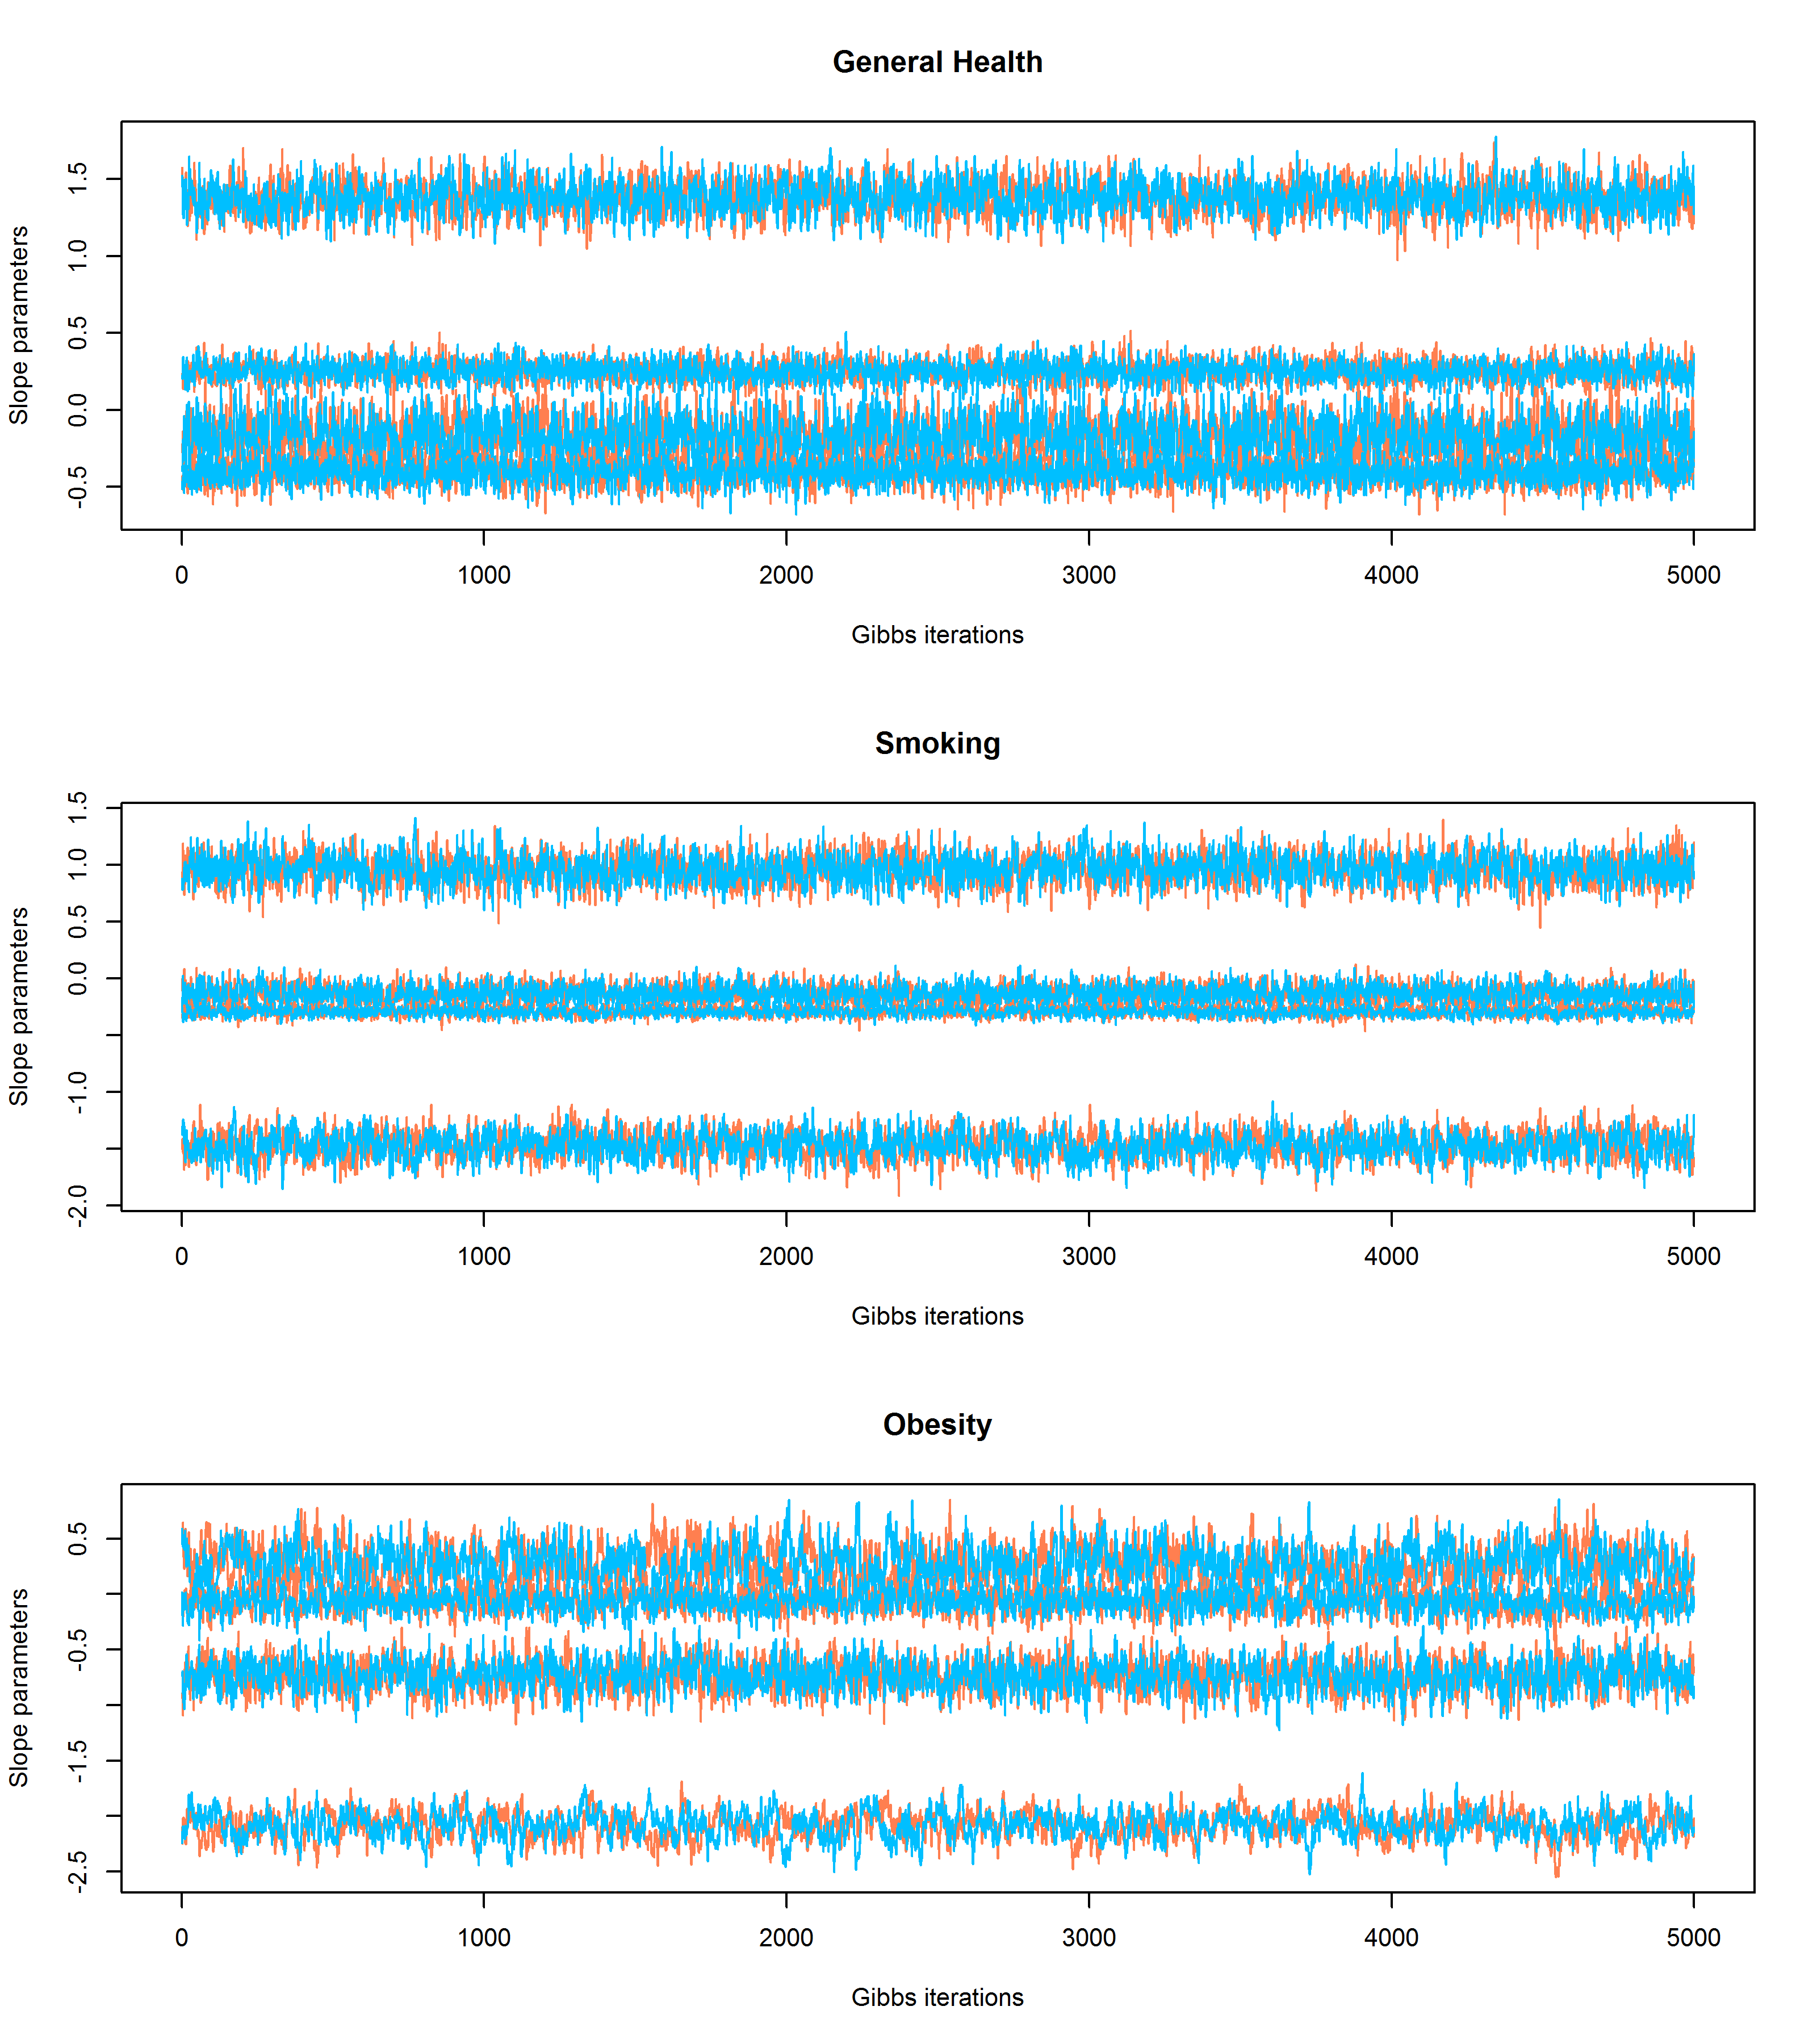
\includegraphics{images/GibbsSvyVar.png}}{}
\makeatother 
\caption{{Gibbs Sampler Draws for the Survey Variable Model Slope Parameters.}}
\label{fig-gibbs-survey-variables}
\end{figure*}
\egroup

\bgroup
\fixFloatSize{images/GibbsRespCost.png}
\begin{figure*}[!htbp]
\centering \makeatletter\IfFileExists{images/GibbsRespCost.png}{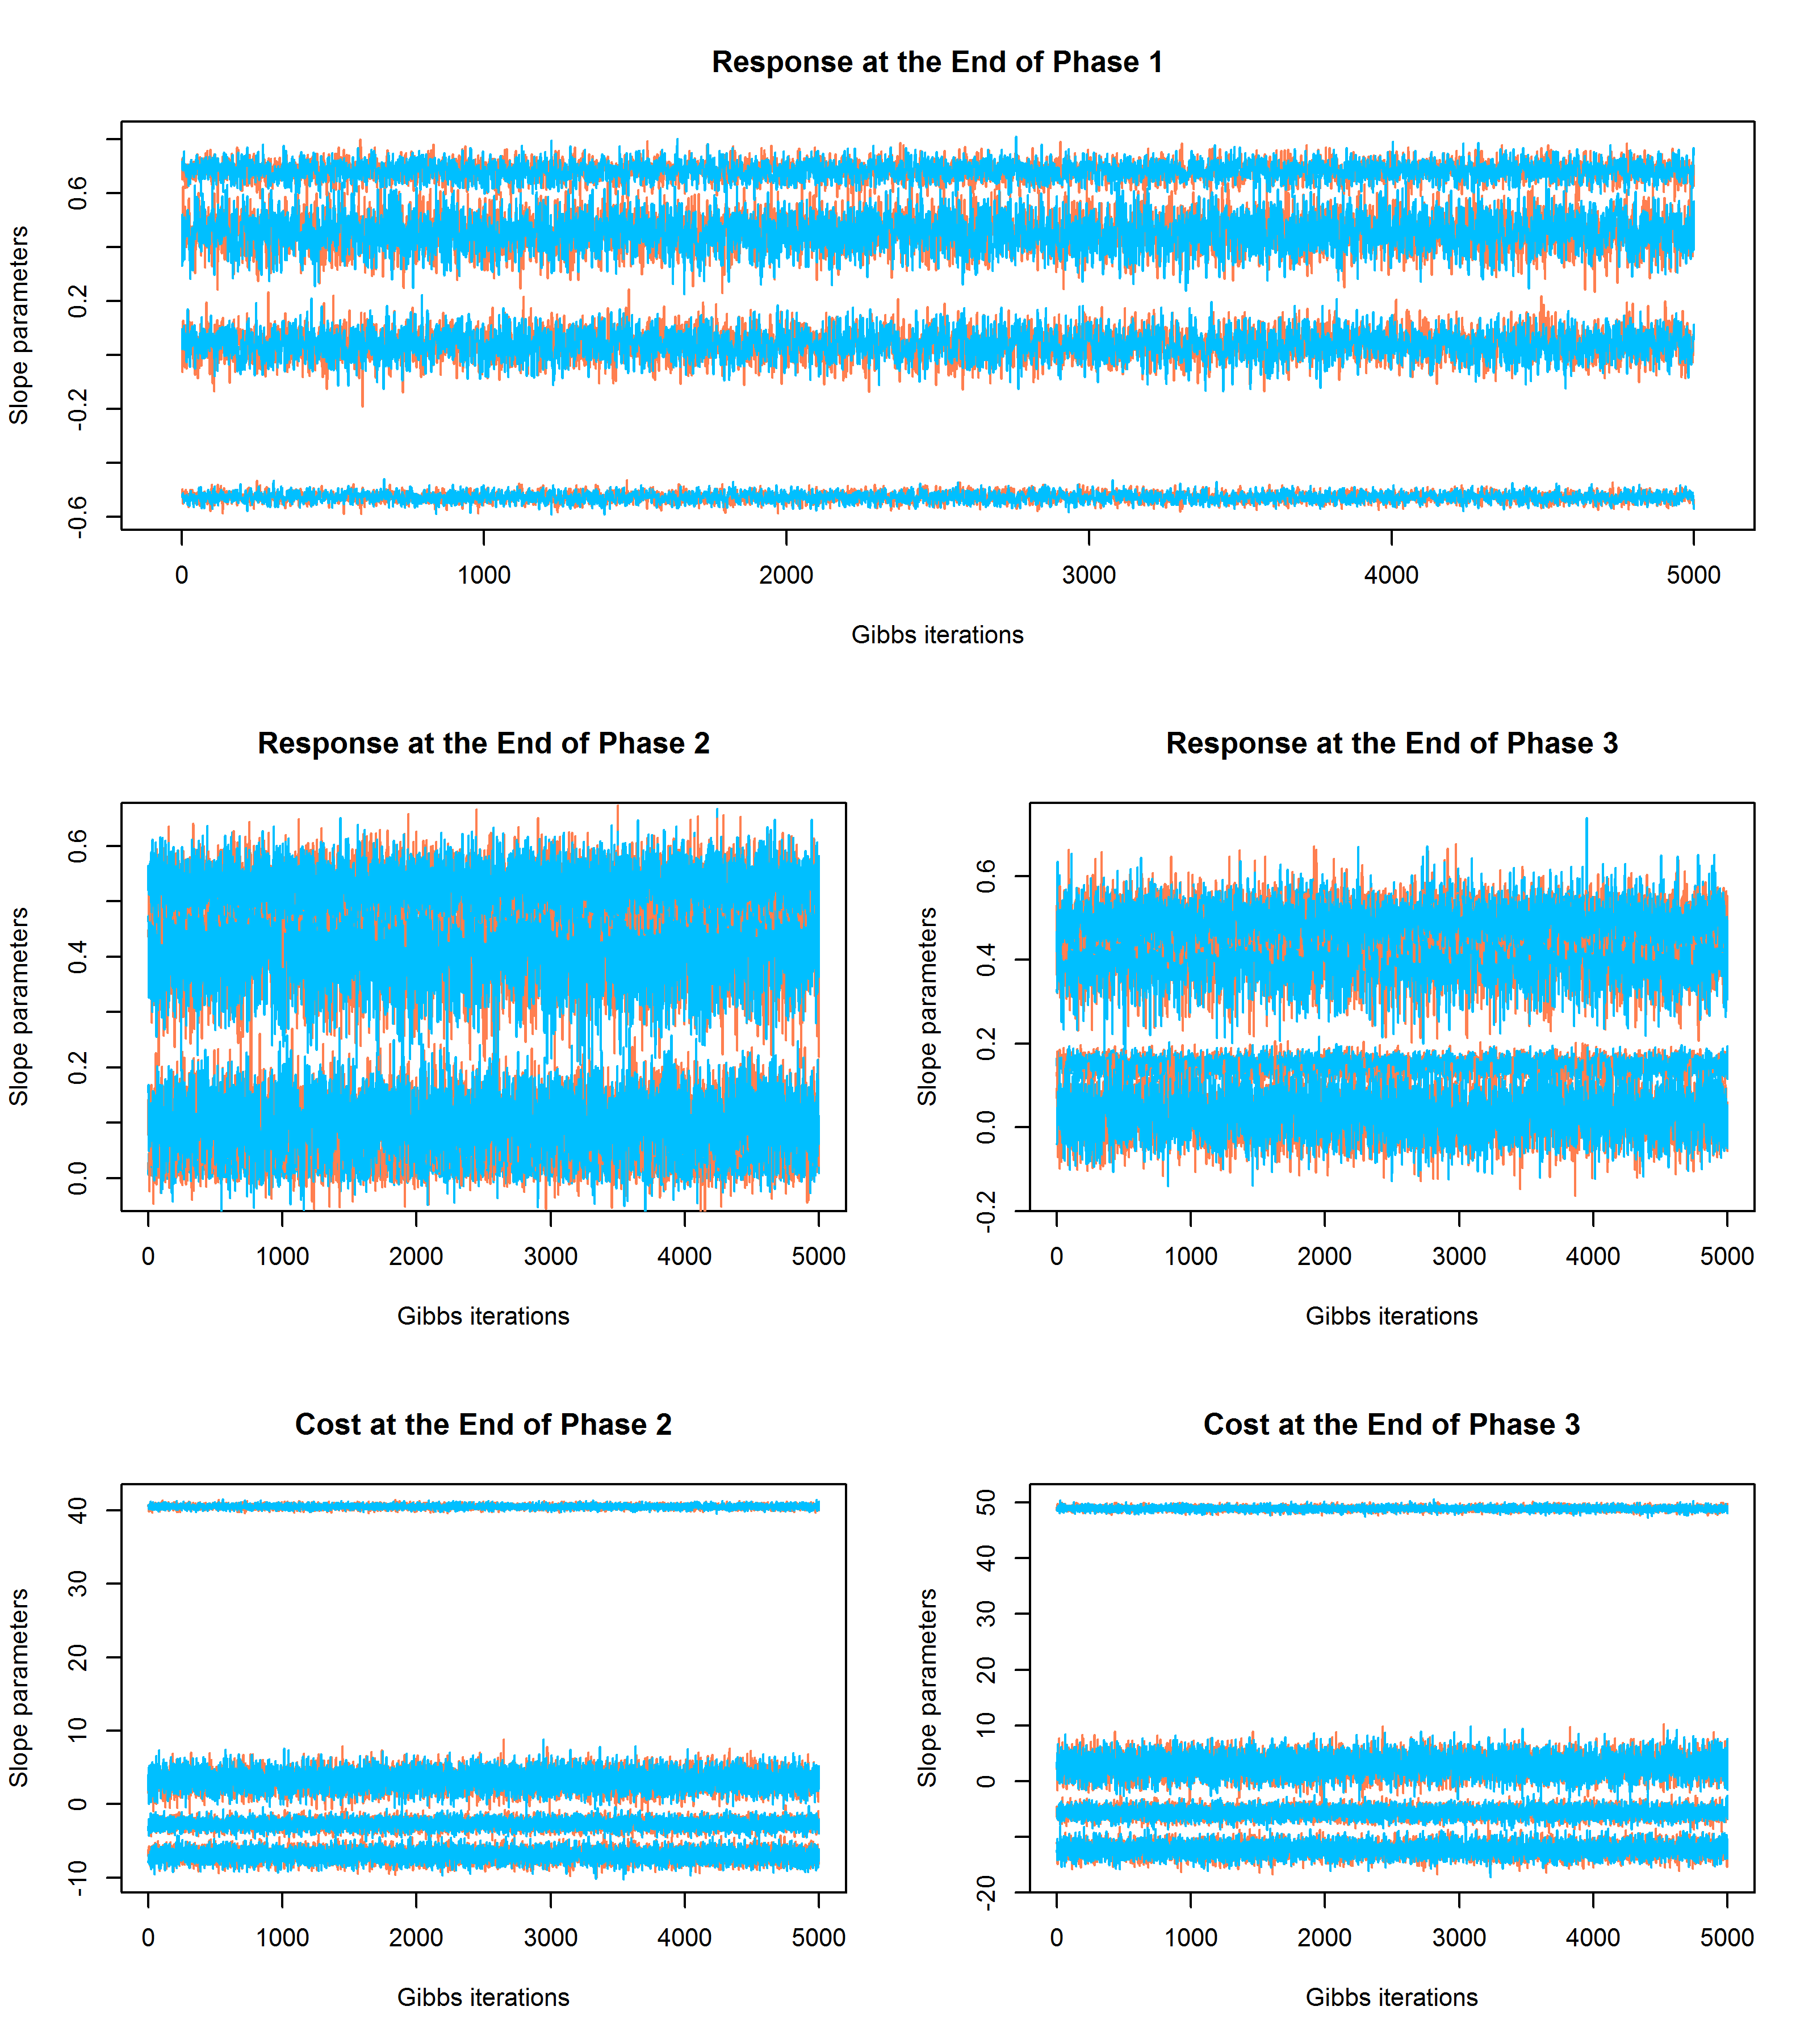
\includegraphics{images/GibbsRespCost.png}}{}
\makeatother 
\caption{{Gibbs Sampler Draws for the Response Propensity and Cost Model Slope Parameters.}}
\label{fig-gibbs-response-cost}
\end{figure*}
\egroup

\bgroup
\fixFloatSize{images/GibbsDesigns.png}
\begin{figure*}[!htbp]
\centering \makeatletter\IfFileExists{images/GibbsDesigns.png}{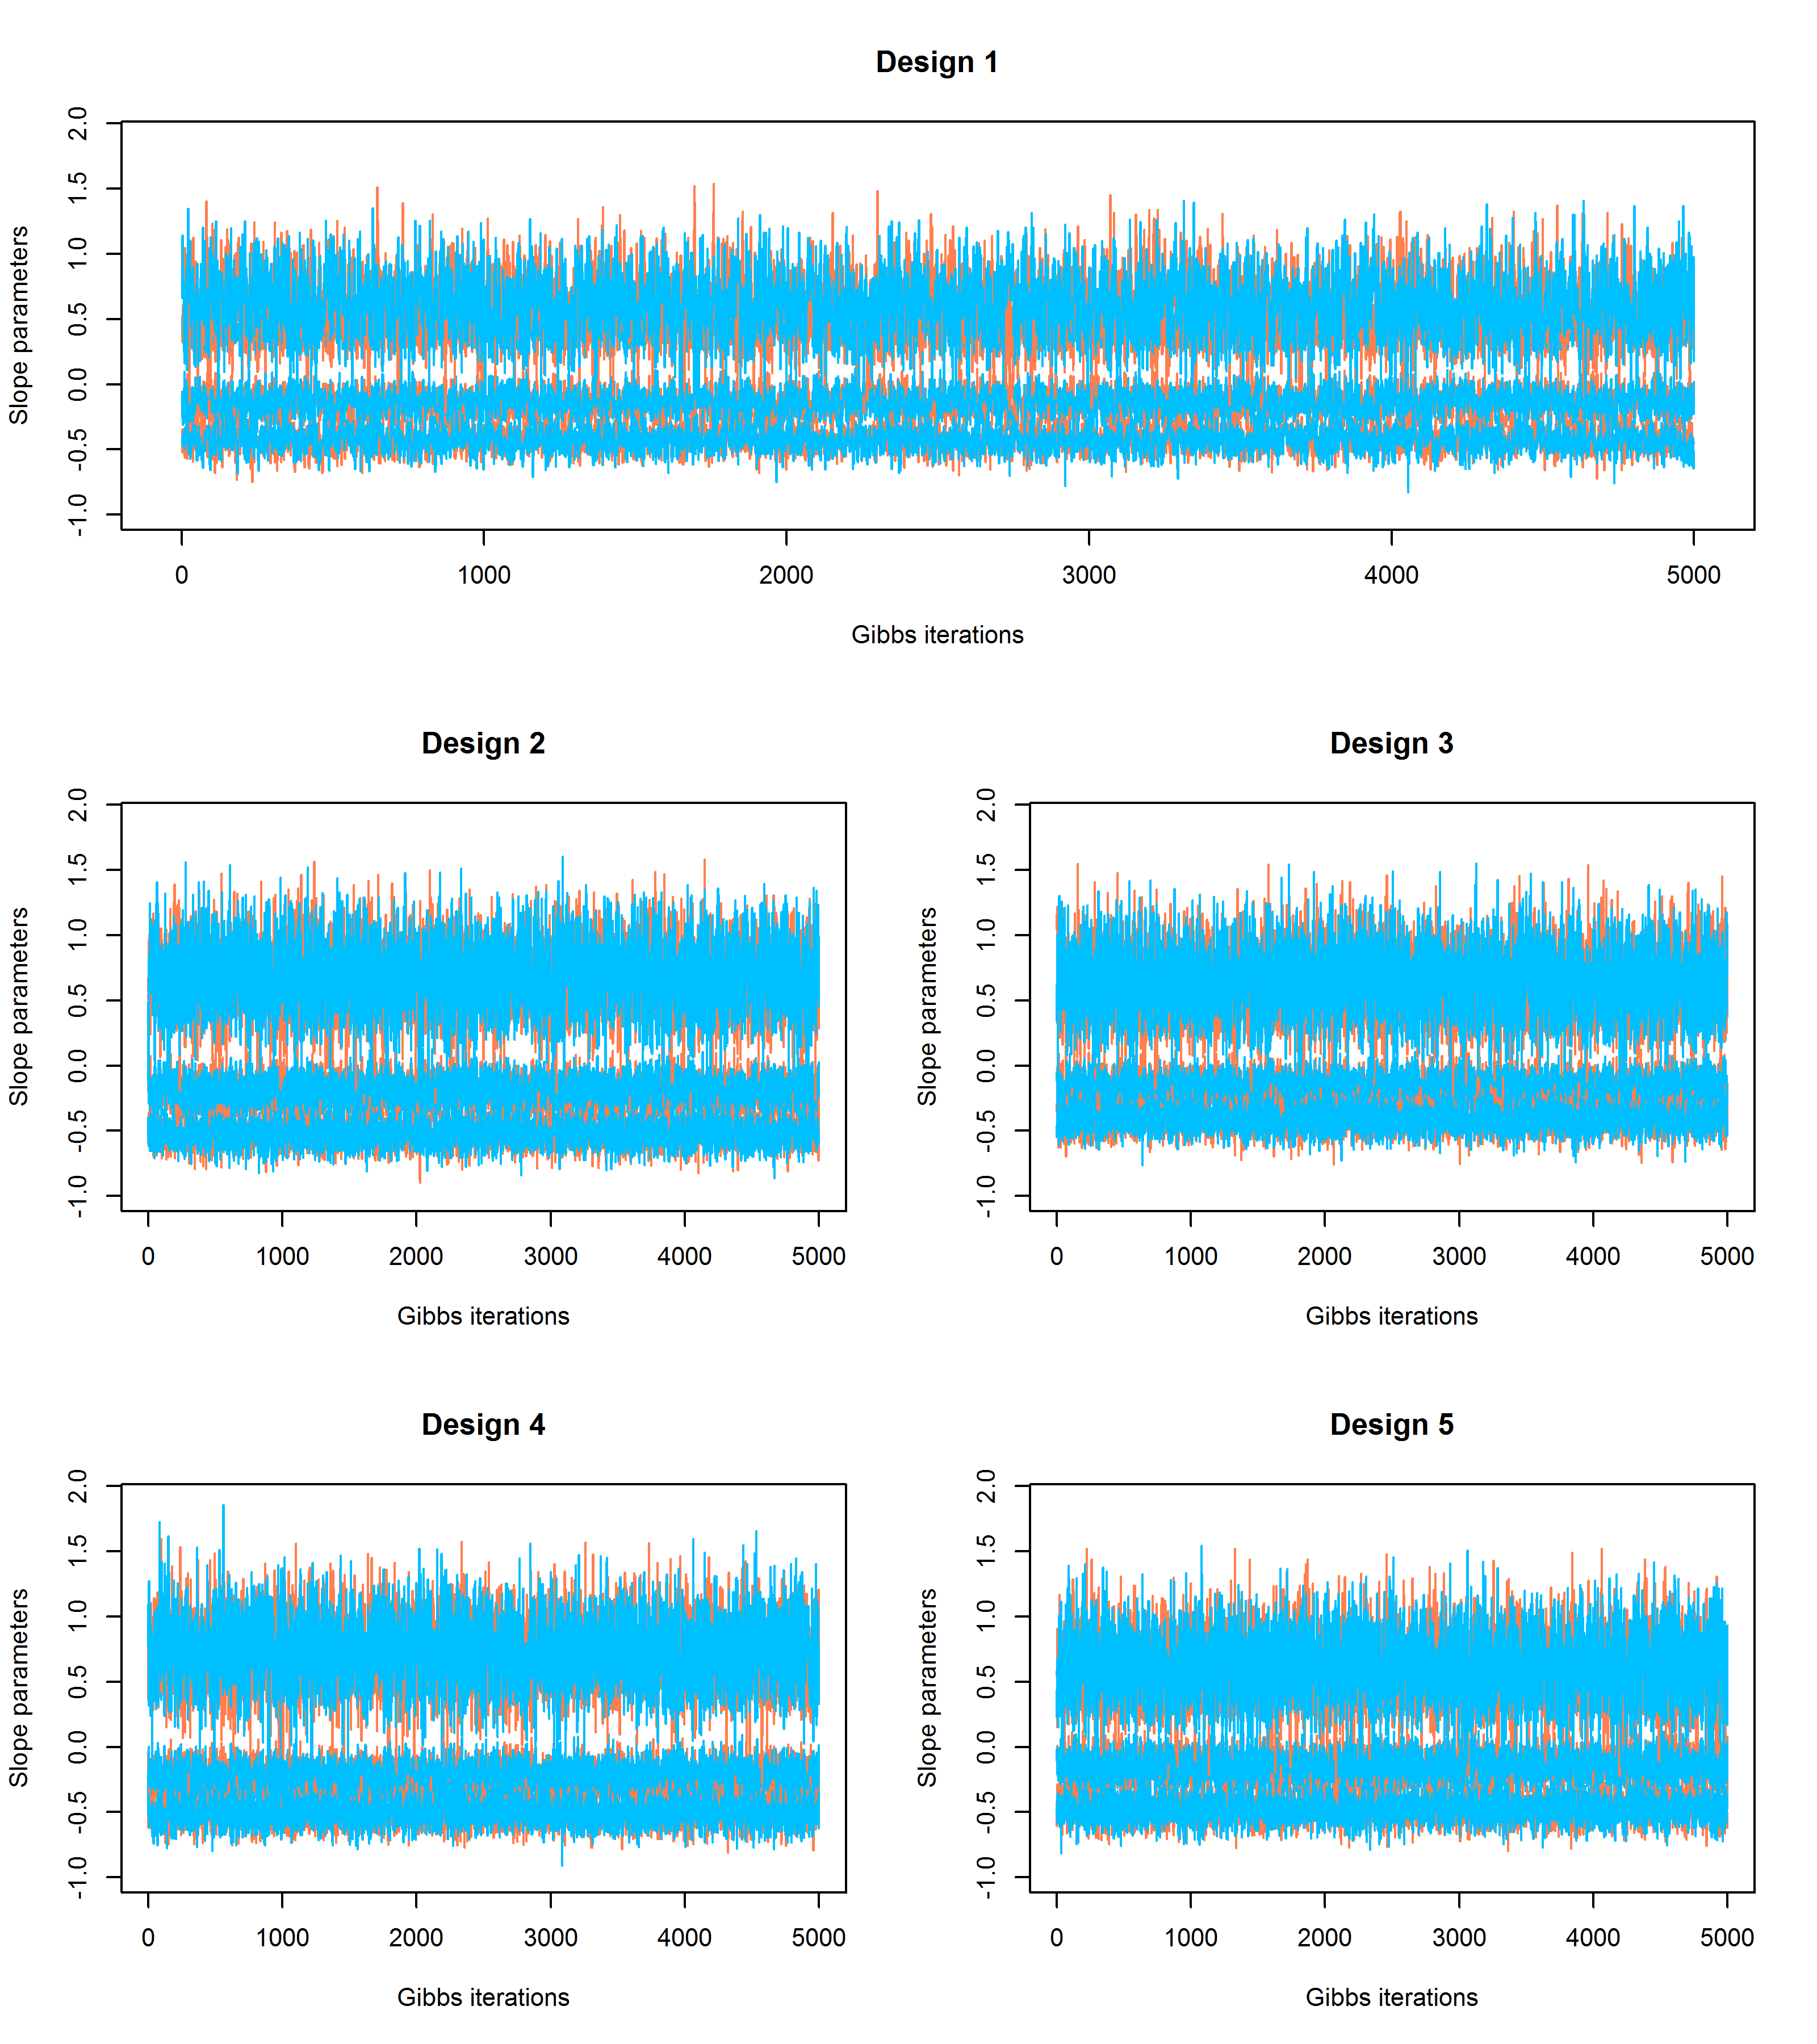
\includegraphics{images/GibbsDesigns.png}}{}
\makeatother 
\caption{{Gibbs Sampler Draws for the Stratification-assessed Response Propensity Model Slope Parameters.}}
\label{fig-gibbs-response-criterion}
\end{figure*}
\egroup

\end{appendices}

\clearpage

\bibliographystyle{ECA_jasa}

\bibliography{article}

\end{document}
